%!TEX TS-program = pdflatex                                          %
%!TEX encoding = UTF8                                                %
%!TEX spellcheck = en-US                                             %
%
%%%%%%%%%%%%%%%%%%%%%%%%%%%%%%%%%%%%%%%%%%%%%%%%%%%%%%%%%%%%%%%%%%%%%%
% Handout_UI_BuildYourOwnBrainNetworkModel.tex
% A handout to follow during the hands-on session 1
% 
% Author: Paula Sanz Leon
% 
% 
%%%%%%%%%%%%%%%%%%%%%%%%%%%%%%%%%%%%%%%%%%%%%%%%%%%%%%%%%%%%%%%%%%%%%%
% based on the tufte-latex template                                  %

\documentclass{tufte-handout}

%\geometry{showframe}% for debugging purposes -- displays the margins

\usepackage{amsmath}

% Set up the images/graphics \underline{\textbf{Analysis}}
\usepackage[pdftex]{graphicx}
\setkeys{Gin}{width=\linewidth,totalheight=\textheight,keepaspectratio}
\graphicspath{{figures/} {../../framework_tvb/tvb/interfaces/web/static/style/img/} {../../framework_tvb/tvb/interfaces/web/static/style/img/nav/}{../../framework_tvb/tvb/interfaces/web/static/style/nodes/}}

\title{The Virtual Brain: Hands on Session \#1}
\date{7th June 2014} 

% The following package makes prettier tables.  
\usepackage{booktabs}


% The units package provides nice, non-stacked fractions and better spacing
% for units.
\usepackage{units}
\usepackage[svgnames]{xcolor}

% The fancyvrb package lets us customize the formatting of verbatim
% environments.  We use a slightly smaller font.
\usepackage{fancyvrb}
\fvset{fontsize=\normalsize}

% Small sections of multiple columns
\usepackage{multicol}

% For adjustwidth environment
\usepackage[strict]{changepage}

% For formal definitions
\usepackage{framed}

% And some maths
\usepackage{amsmath}  % extended mathematics

% Resume a list
\usepackage{enumitem}

% Background image

\usepackage{wallpaper}

% Provides paragraphs of dummy text
\usepackage{lipsum}

% These commands are used to pretty-print LaTeX commands
\newcommand{\doccmd}[1]{\texttt{\textbackslash#1}}% command name -- adds backslash automatically
\newcommand{\docopt}[1]{\ensuremath{\langle}\textrm{\textit{#1}}\ensuremath{\rangle}}% optional command argument
\newcommand{\docarg}[1]{\textrm{\textit{#1}}}% (required) command argument
\newenvironment{docspec}{\begin{quote}\noindent}{\end{quote}}% command specification environment
\newcommand{\docenv}[1]{\textsf{#1}}% environment name
\newcommand{\docpkg}[1]{\texttt{#1}}% package name
\newcommand{\doccls}[1]{\texttt{#1}}% document class name
\newcommand{\docclsopt}[1]{\texttt{#1}}% document class option name

\newcommand\blfootnote[1]{\begingroup
         \renewcommand\thefootnote{}\footnote{\phantom{\thefootnote} #1}%
         \addtocounter{footnote}{-1}%
         \endgroup
          }

% Colours: environment derived from framed.sty: see leftbar environment definition
\definecolor{formalshade}{rgb}{0.95,0.95,1}
\definecolor{simulationshade}{rgb}{0.92, 1.0, 0.95}

% Title rule
\newcommand{\HRule}{\rule{\linewidth}{0.5mm}}

% Framed  coloured boxes

%% Blue box: for steps regarding analysis and such
\newenvironment{formal}{%
  \def\FrameCommand{%
    \hspace{1pt}%
    {\color{DarkBlue}\vrule width 2pt}%
    {\color{formalshade}\vrule width 4pt}%
    \colorbox{formalshade}%
  }%
  \MakeFramed{\advance\hsize-\width\FrameRestore}%
  \noindent\hspace{-4.55pt}% disable indenting first paragraph
  \begin{adjustwidth}{}{7pt}%
  \vspace{2pt}\vspace{2pt}%
}
{%
  \vspace{2pt}\end{adjustwidth}\endMakeFramed%
}

%% Green box: for steps regarding simulatio **only**
\newenvironment{simulation}{%
  \def\FrameCommand{%
    \hspace{1pt}%
    {\color{ForestGreen}\vrule width 2pt}%
    {\color{simulationshade}\vrule width 4pt}%
    \colorbox{simulationshade}%
  }%
  \MakeFramed{\advance\hsize-\width\FrameRestore}%
  \noindent\hspace{-4.55pt}% disable indenting first paragraph
  \begin{adjustwidth}{}{7pt}%
  \vspace{2pt}\vspace{2pt}%
}
{%
  \vspace{2pt}\end{adjustwidth}\endMakeFramed%
}

%% Orange box: for verbose descriptions
\newenvironment{blah}{%
  \def\FrameCommand{%
    \hspace{1pt}%
    {\color{DarkOrange}\vrule width 2pt}%
    {\color{PeachPuff}\vrule width 4pt}%
    \colorbox{PeachPuff}%
  }%
  \MakeFramed{\advance\hsize-\width\FrameRestore}%
  \noindent\hspace{-4.55pt}% disable indenting first paragraph
  \begin{adjustwidth}{}{7pt}%
  \vspace{2pt}\vspace{2pt}%
}
{%
  \vspace{2pt}\end{adjustwidth}\endMakeFramed%
}

\begin{document}
\thispagestyle{plain}
\LLCornerWallPaper{1.5}{background.png}
\begin{titlepage}
\begin{center}
% Upper part of the page. The '~' is needed because \\
% only works if a paragraph has started.

\includegraphics[width=1.5\textwidth]{./tvb_logo_transparent_square.png}~\\[0.5cm]

% Title
\begin{fullwidth}
\HRule \\[0.2cm]
\begin{center}
{ \huge \bfseries Hands-on Session \#1 \\ [0.2cm] Building Your Own Brain Network Model \\[0.1cm] }
{ \large \bfseries June 7, 2014 \\[0.2cm]}
\end{center}
\HRule \\[0.2cm]
\end{fullwidth}

\end{center}
\end{titlepage}
\newpage
\ClearWallPaper
\begin{abstract}
\noindent TVB allows for a systematic exploration and manipulation of every
underlying component of a large-scale brain network model, such as the neural
mass model governing the local dynamics \sidenote{There are a number of predefined models available in TVB} or the structural connectivity
constraining the space-time structure of the network couplings.
\begin{marginfigure}%
  %
\includegraphics[width=\linewidth]{tvb_logo_transparent_square}
  %\caption{TVB evil logo}
  \label{fig:marginfig}
\end{marginfigure}
\end{abstract}

%\printclassoptions

%\begin{fullwidth} % uncomment this environment to get full texwidth paragraphs 
%\textsc{The Virtual Brain} is a facilitating technology. It enables
%researchers from the domains of  computational neuroscience and medicine to
%study and focus on a particular problem, and directly build a model of the
%brain that can be tested under different scenarios. So, every time we require
%to perform a simulation for our work, we do not require to develop the
%underlying computational model.   
%\end{fullwidth}

\section{Objectives}\label{sec:objectives}

\newthought{This tutorial presents} the basic anatomy of a brain network model at the region level using The
Virtual Brain's (TVB's) graphical interface. You are not expected to launch all the simulations. However, following these steps you should
be able to reproduce the results from the simulations in the project Building
Your Own Brain Network Model. 

\section{Project:  Session\_I\_BuildingYourOwnBrainNetworkModel}\label{sec:project_data}

\begin{margintable}
  \centering
  \fontfamily{ppl}\selectfont
  \begin{tabular}{l}
    \toprule
    Name \\
    \midrule
    \multicolumn{1}{l}{Building A Discrete Brain Network Model }\\
    $\quad$ \textit{AnatomyOfARegionSimulation\_a} \\
    $\quad$\textit{AnatomyOfARegionSimulation\_b}  \\ 
    \\
    \multicolumn{1}{l}{Looking At The Results}\\
    \\
    \multicolumn{1}{l}{Parameter Space Exploration}\\
     $\quad$\textit{AnatomyOfARegionSimulation\_pse\_a} \\
    \\
    \multicolumn{1}{l}{Simulation Continuation or branching}\\
     $\quad$\textit{AnatomyOfARegionSimulation\_a\_branch1} \\
    \\
    \multicolumn{1}{l}{Stochastic Simulations}\\
     $\quad$\textit{AnatomyOfARegionSimulation\_c}  \\
    \\
    \multicolumn{1}{l}{Extra}\\
     $\quad$\textit{AnatomyOfARegionSimulation\_d}  \\ 
     $\quad$\textit{AnatomyOfARegionSimulation\_d\_branch1}  \\ 
    \\
     \multicolumn{1}{l}{Modelling the Neural Activity}\\
     \multicolumn{1}{l}{On the Folded Cortex}\\
    $\quad$\textit{AnatomyOfASurfaceSimulation} \\
    $\quad$\textit{AnatomyOfASurfaceSimulation\_branch1}
    \\
    \multicolumn{1}{l}{Define Your Own Local Connectivity}\\
      $\quad$\textit{SurfaceSimulation\_GaussianLocalConnectivity} \\
      $\quad$\textit{SurfaceSimulation\_MexicanHatLocalConnectivity}\\
    \bottomrule
  \end{tabular}
  \caption{Simulations in this project.}
  \label{tab:normaltab}
\end{margintable}


% let's start a new thought -- a new section
\newthought{In this project}, all the data were already generated. We'll only go through the necessary steps required to reproduce some simulations listed in Table~\ref{tab:normaltab}. You can always start over, click along and/or try to change parameters.


\subsection{Building A Discrete Brain Network Model}\label{sec:region_simulations}

\newthought{A basic simulation} at the region level uses a coarse representation of the brain and consists of
five main components, each of these components is a configurable object in
TVB:
\begin{blah}
\begin{itemize}
\item \underline{Model} or \underline{Local population model}, which is, at its core, a set of differential equations describing the local neuronal dynamic;
\item \underline{Connectivity}, represents the large scale structural connectivity of the brain, ie white-matter tracts;
\item \underline{Long range Coupling}, is a function that is used to join the local \underline{Model} dynamics at distinct locations over the connections described in \underline{Connectivity};
\item \underline{Integrator}, is the integration scheme that will be applied to the coupled set of differential equations;
\item \underline{Monitors}, one or more \underline{Monitors} can be attached to a simulation, they act to record the output data.
\end{itemize}
\end{blah}

\begin{figure}[h]
  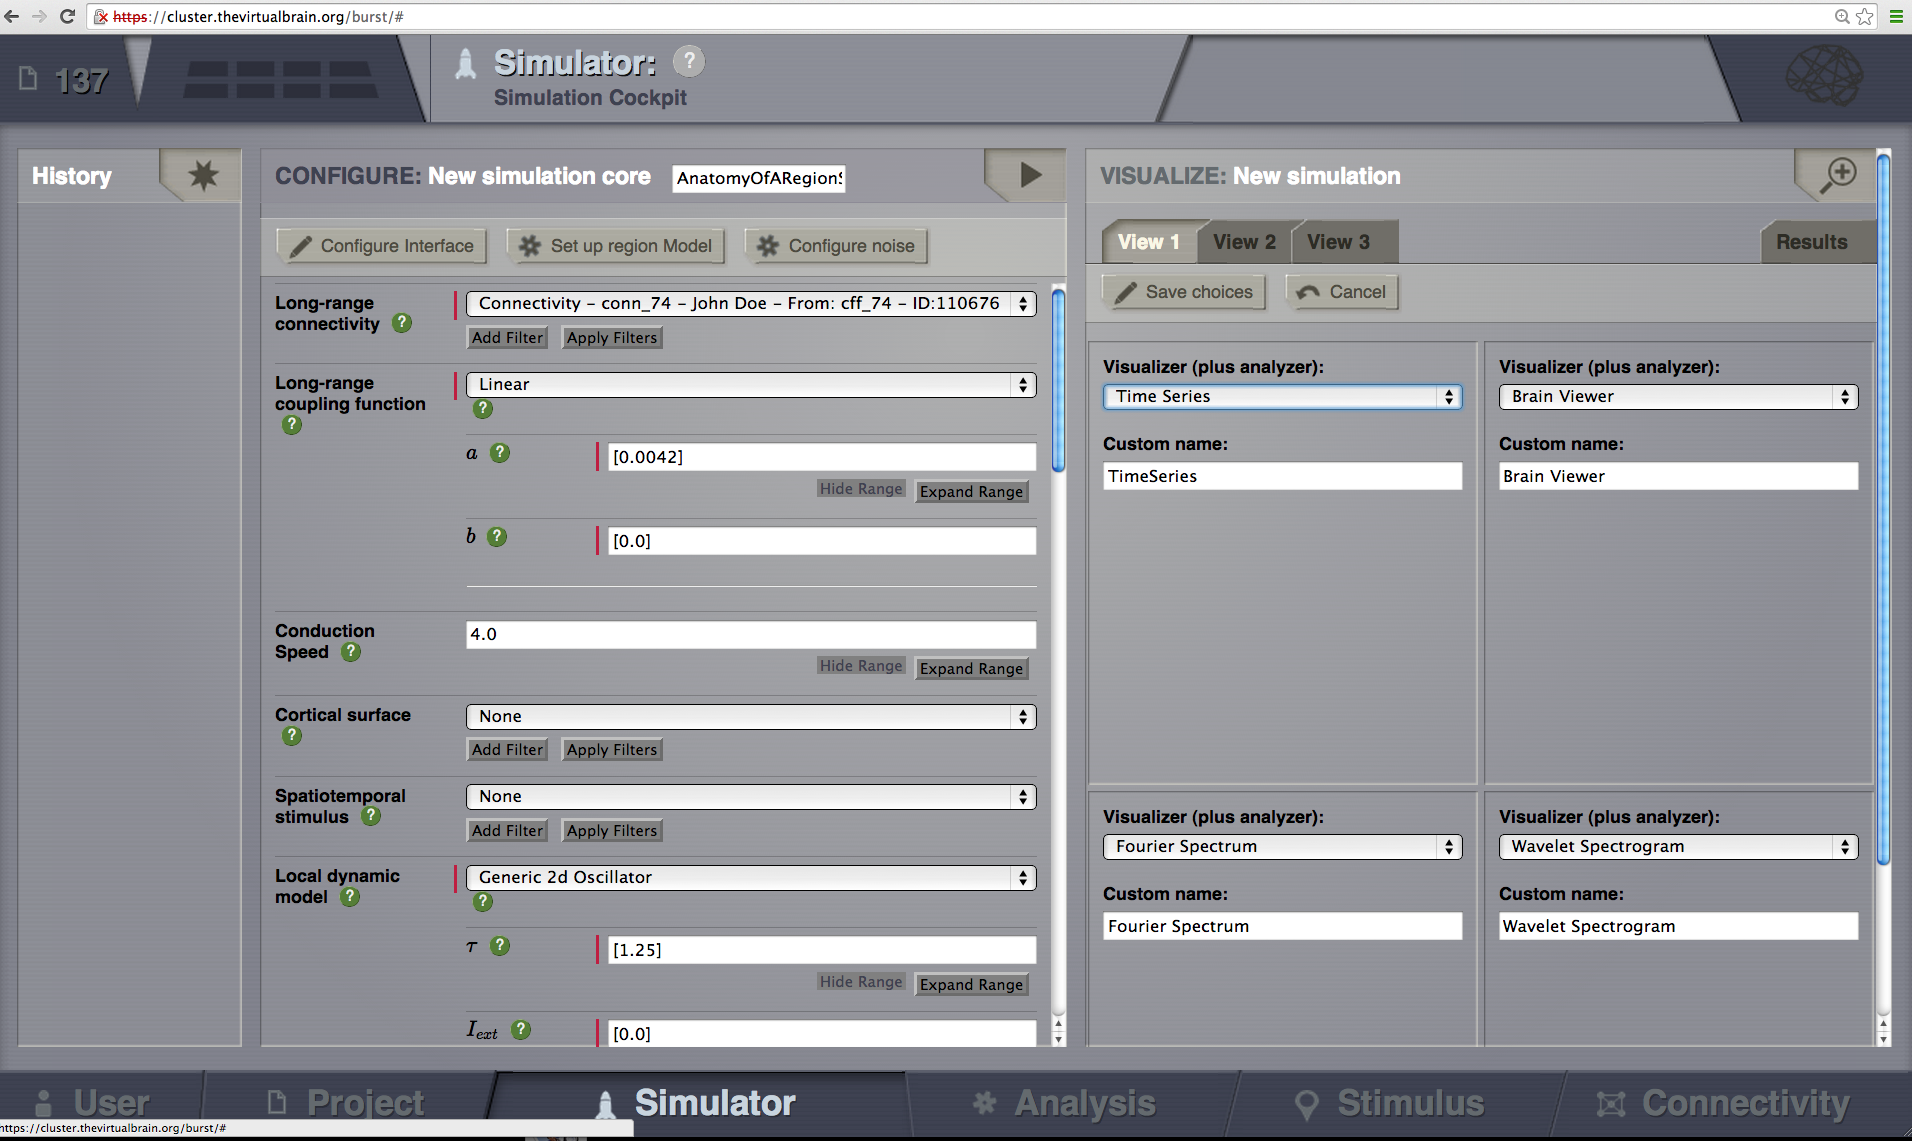
\includegraphics[width=\linewidth]{Handout_UI_BuildingYourOwnBrainNetworkModel_SimulatorArea}%
  \caption{TVB's \textsc{Simulator} page}%
  \label{fig:fig}%
\end{figure}

In this example, \textit{AnatomyOfARegionSimulation\_a}, we will change the default parameters and configure some
visualizers on the right column to have a quick idea of some properties of the
simulated data.
\begin{simulation}
\begin{enumerate}
\item Go to the \textsc{simulator} page. (Fig.~\ref{fig:fig})

\item \underline{Connectivity:} Define some structure for your network. Here, we'll rely on \textbf{TVB's default  matrix.} 

\item Set a \underline{Long range coupling} function. For our present purposes, we happen to know that for the parameters we will use through TVB's default \underline{Connectivity} matrix, a linear function with a slope of $\mathbf{a=0.0042}$ is a reasonable thing to use. 

\item \underline{Conduction speed:} Alter the speed of signal propagation through the network to \textbf{\unitfrac[4]{mm}{ms}}. 

\item \underline{Local dynamics:} Then define a \underline{Model} for the local dynamics . Here we'll use the \textbf{generic 2 dimensional oscillator} (see Fig. \ref{fig:step_01}) with the parameters shown in Table \ref{tab:modeltab}.


\item Now that we've defined our structure and dynamics we need to select an integration scheme. We'll use \textbf{HeunDeterministic}. The most important thing here is to use a step size that is small enough for the integration to be numerically stable. Here, we chose a value of $\mathbf{dt=}$\textbf{\unit[0.1]{ms}}.

\item  Select the \textbf{Temporal Average} monitor. It averages over a time window of length \underline{sampling period} returning one time point every period. It also, by default, only returns those state-variables flagged in the \underline{Models} definition as \underline{Variables watched by Monitors}. For our example the \underline{Monitor's sampling period} is \textbf{\unit[1]{ms}}. 
\end{enumerate}
\end{simulation}

\begin{figure}[h]
  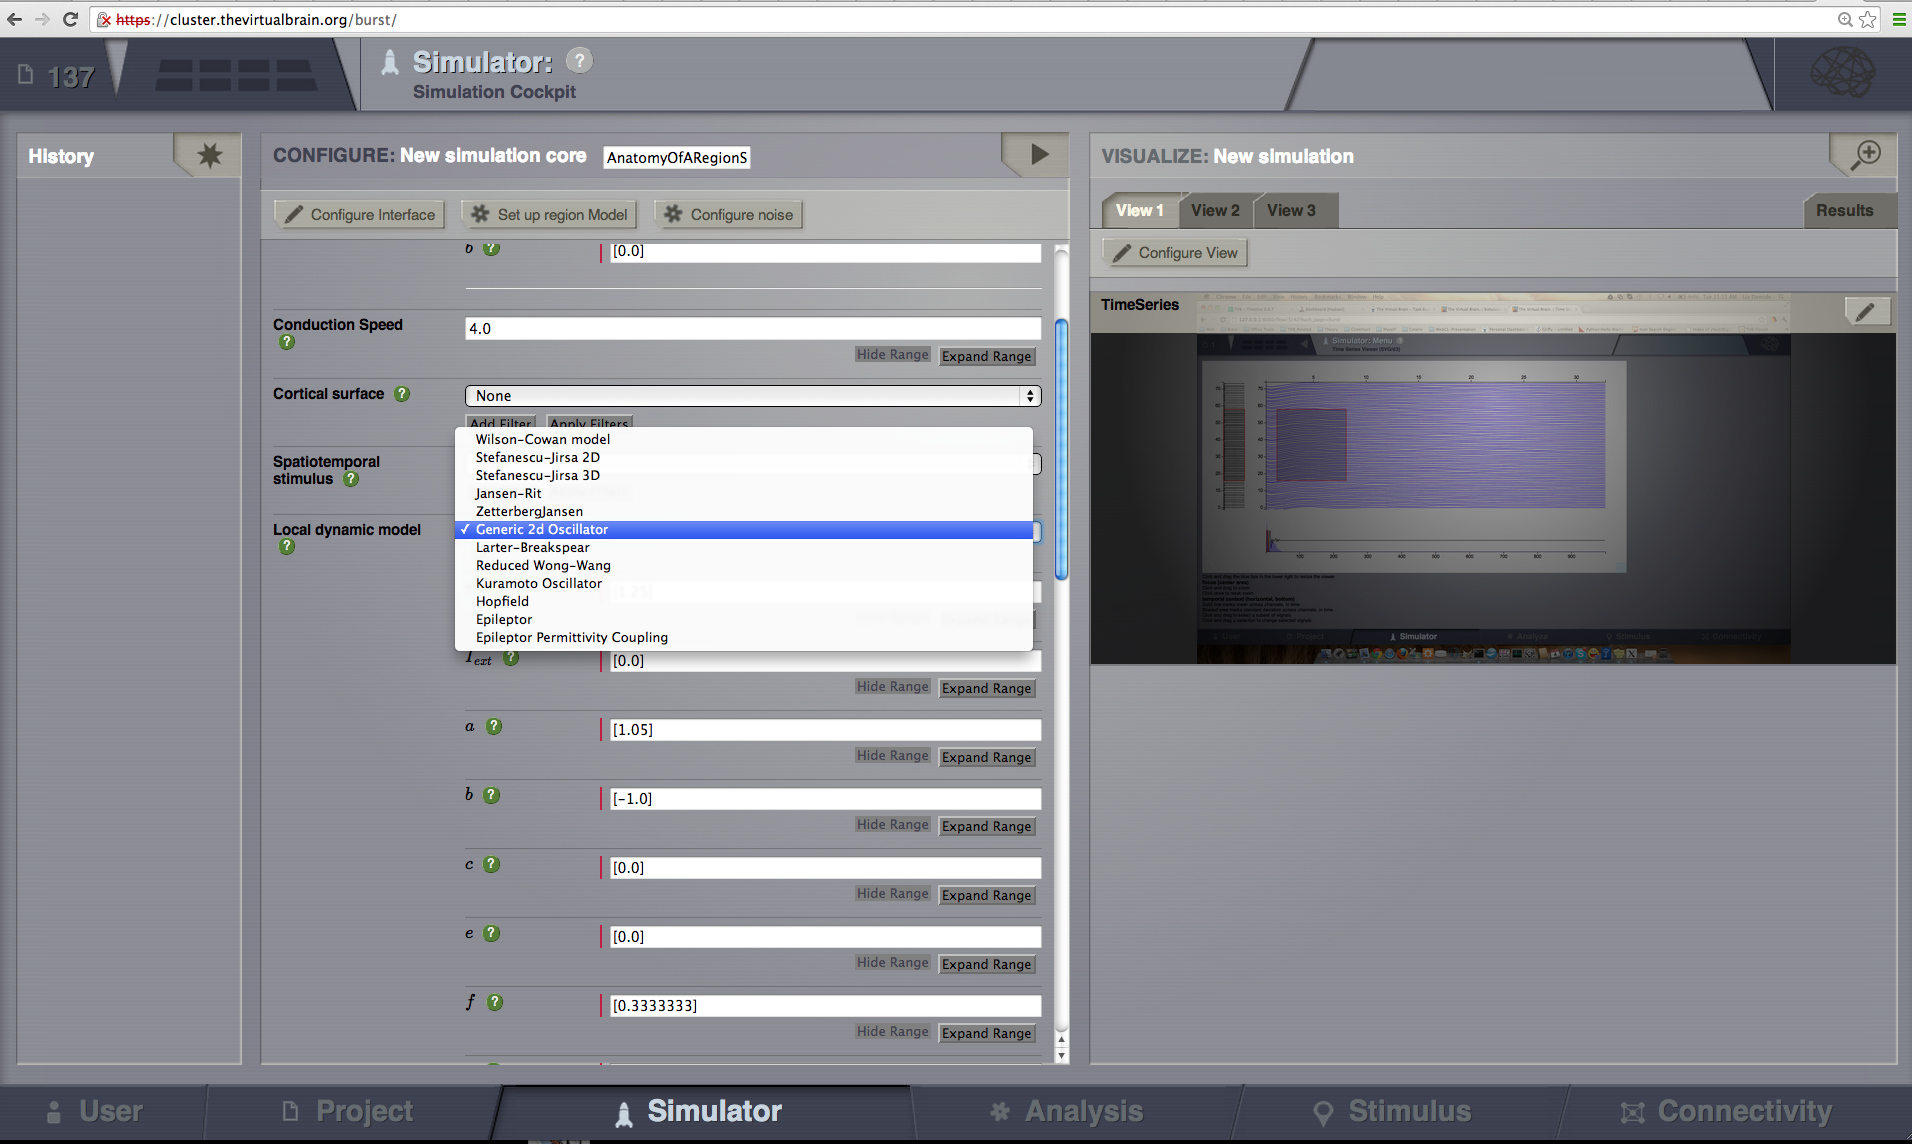
\includegraphics[width=\linewidth]{Handout_UI_BuildingYourOwnBrainNetworkModel_Model}%
  \caption{Selecting a \underline{Model}}%
  \label{fig:step_01}%
\end{figure}


\begin{margintable}
  \centering
  \fontfamily{ppl}\selectfont
  \begin{tabular}{ll}
    \toprule
    Model parameter & Value \\
    \midrule
             $a$          &   1.05   \\
             $b$          &  -1.0    \\
             $c$           &   0        \\
             $d$           &   0.1    \\
             $e$           &   0        \\
             $f$            &   1/3    \\
             $g$           &   1        \\
             $I$            &   0        \\
             $\alpha$   &   1        \\
             $\beta$     &   0.2     \\
             $\gamma$&  -1       \\
             $\tau$       &   1.25   \\
    \bottomrule
  \end{tabular}
  \caption{Generic 2d oscillator parameters}
  \label{tab:modeltab}
\end{margintable}



%The important thing to know here is that TVB doesn't support interpolation of
%the time-series it produces, which means that the period given to a monitor
%must be an integral multiple of the time step size, \underline{dt}, selected for the integration scheme.

Although there are Monitors which apply a biophysical measurement process to
the simulated neural activity, such as EEG, MEG, SEEG, etc.,  here we'll select only
one simple monitor just to show the idea. The Raw Monitor takes no arguments
and simply returns all the simulated data. \sidenote{As a general rule this monitor
shouldn't be used for anything but very short simulations as the amount of
data returned can become prohibitively large.}


\begin{simulation}
\begin{enumerate}[resume]
  \setcounter{enumi}{7}
 \item Provide the \underline{simulation length}, that here we'll use the default value of \textbf{\unit[1000]{ms}}.
 \item Before launching the simulation, configure a set of \underline{Visualizers} and/or \underline{Analyzers} by clicking on \underline{Configure}, selecting the what you want to see and saving your choices. (see Table \ref{tab:portletstab}). These windows will enable you to have a glimpse of the results as soon as the simulation ends. 
 \item Enter a name for the current simulation (e.g, \textit{AnatomyOfARegionSimulation\_a}) and click on  
\includegraphics[width=0.025\textwidth]{butt_launch_project.png}.
\end{enumerate}
\end{simulation}

\begin{margintable}
  \centering
  \fontfamily{ppl}\selectfont
  \begin{tabular}{ll}
    \toprule
    Window & Visualizer/Analyzer \\
    \midrule
             top-left          &   Time Series   \\
             top-right        &   Brain Viewer\\
             bottom-left    &   Fourier Transform        \\
             bottom-right  &   Wavelet Spectrogram \\
    \bottomrule
  \end{tabular}
  \caption{Selected visualizers. It is possible to configure up to 12 different windows. }
  \label{tab:portletstab}
\end{margintable}


\subsection{Looking at the Results}\label{sec:results}

\newthought{The transient large} amplitude oscillatory activity at the beginning of the
simulation (see Fig. \ref{fig:time_series}) is a result of the imperfectly set initial conditions.

\begin{figure}[h]
  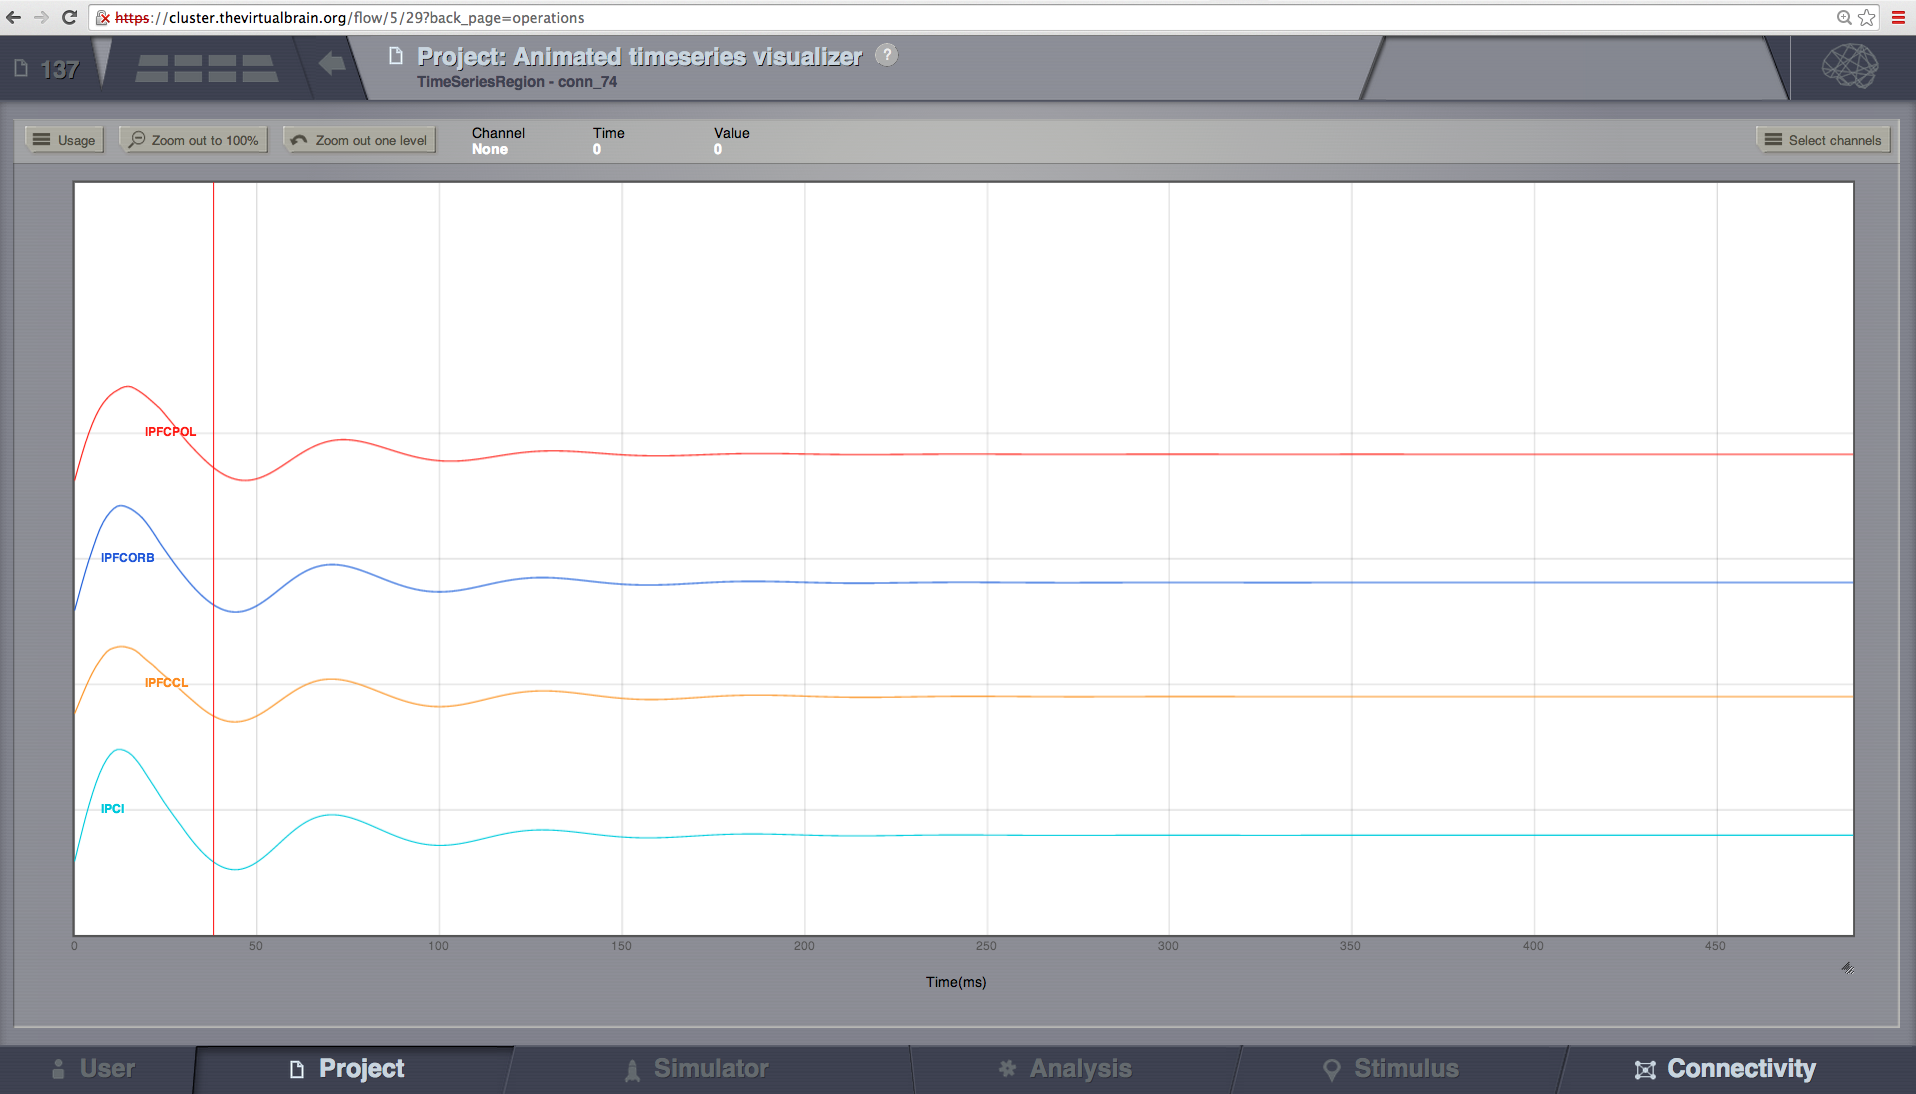
\includegraphics[width=\linewidth]{Handout_UI_BuildingYourOwnBrainNetworkModel_AnimatedTimeSeries}%
  \caption{Time-series from \textit{AnatomyOfARegionSimulation\_a}}%
  \label{fig:time_series}%
\end{figure}
 
\begin{blah}
The initial history (i.e., initial conditions) is
merely set by default to be random walks within the general \underline{range of state-variable values} expected from the model. 
As the current simulation is
configured with fixed point dynamics, if we were to set the initial conditions
exactly to the values corresponding to that fixed point there would be no such
initial transient (we will see how to achieve that later on).
\end{blah}


\begin{formal}
\begin{enumerate}
\item Go to \textsc{Projects} $\rightarrow$ \textsc{operations dashboard}.
\item Click on the icon of the time-series 
\includegraphics[width=0.05\textwidth]{nodeTimeSeriesRegion.png}. From the metadata overlay's visualizers tab, launch the \underline{Animated Time Series Visualizer}.
\item Go back to the \textsc{simulator} page and check the Fourier spectrum. Select a linear scale on the Y axis. We see that the intrinsic frequency of the oscillations is set at about \unit[11]{Hz} (see Fig. \ref{fig:fourier}). 
\end{enumerate}
\end{formal}

\begin{figure}[h]
  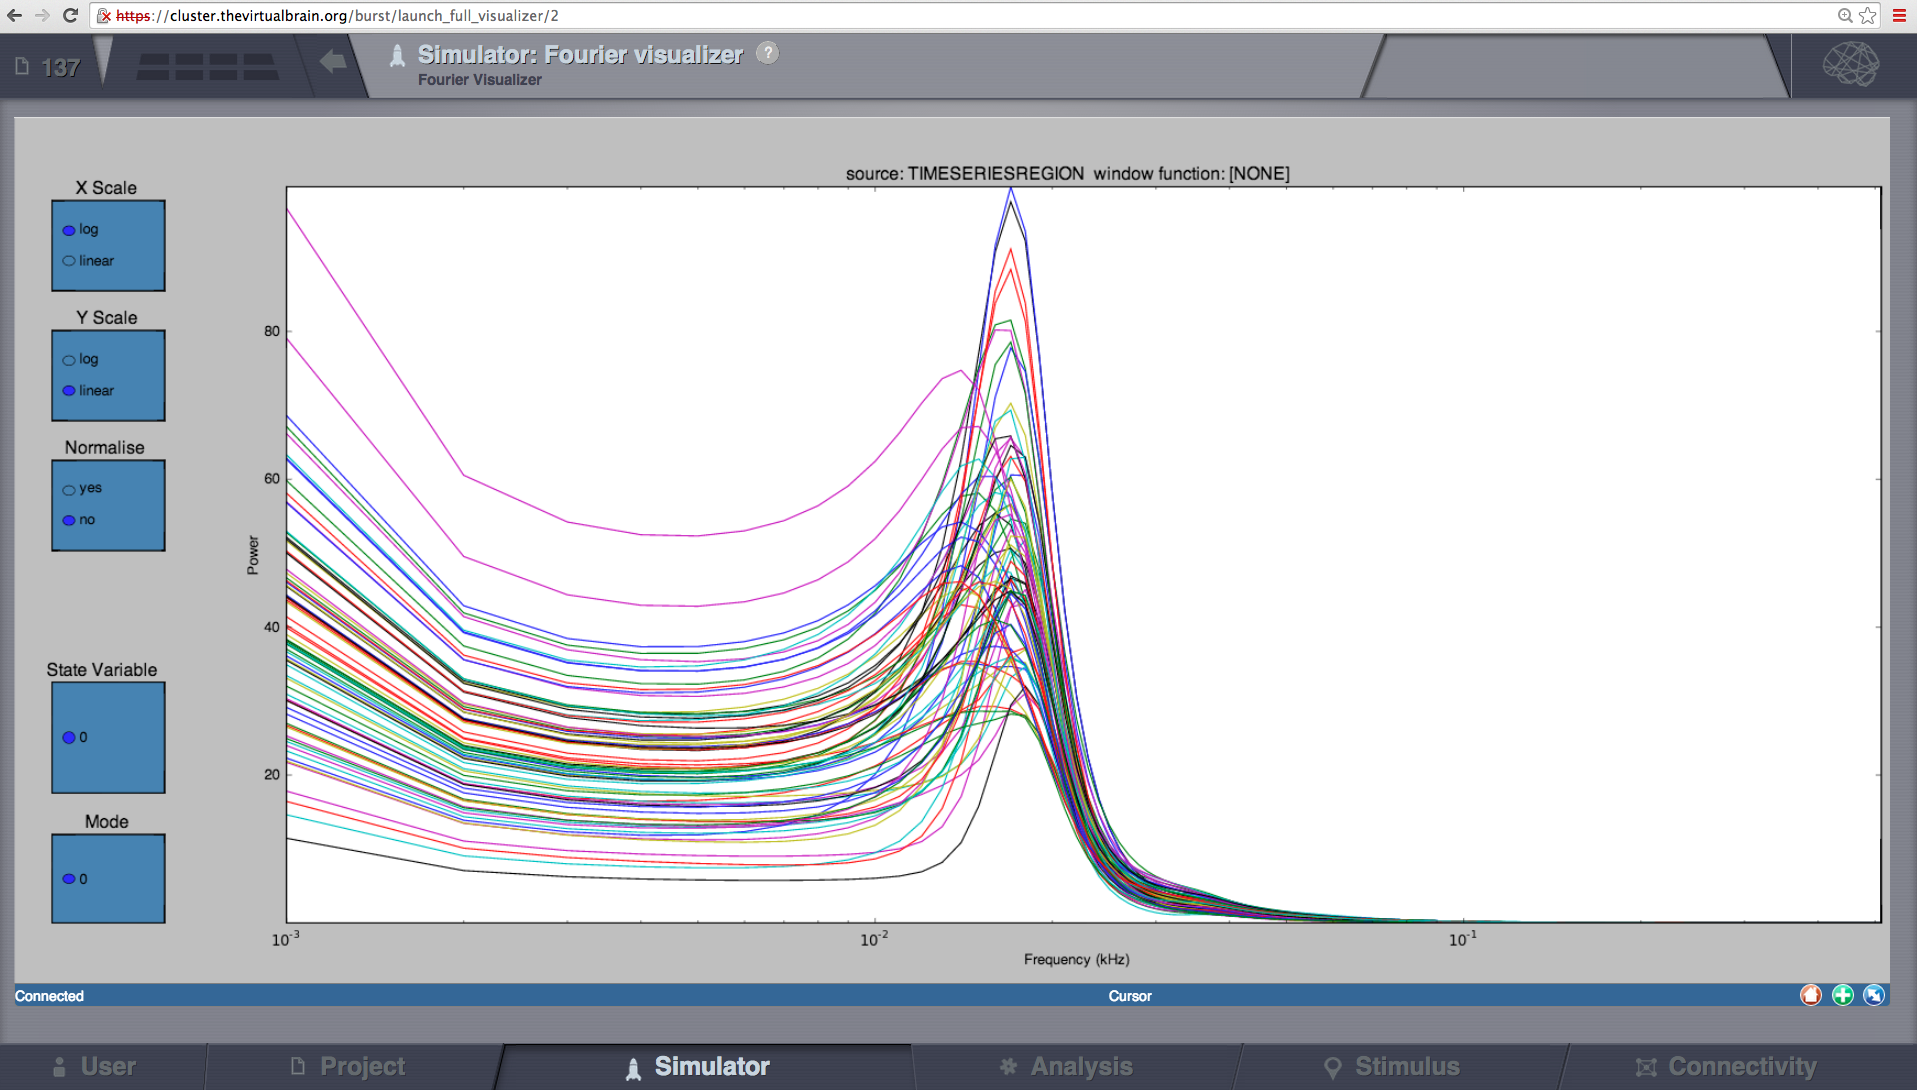
\includegraphics[width=\linewidth]{Handout_UI_BuildingYourOwnBrainNetworkModel_Fourier}%
  \caption{Fourier spectra of the time-series from \textit{AnatomyOfARegionSimulation\_a}}%
  \label{fig:fourier}%
\end{figure}


\begin{marginfigure}
  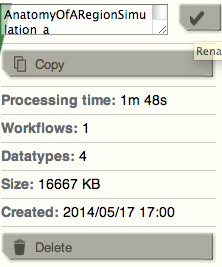
\includegraphics[width=\linewidth]{Handout_UI_BuildingYourOwnBrainNetworkModel_CopyASimulation}
  \caption{Copy a simulation.}%
  \label{fig:sim_copy}%
\end{marginfigure}

\begin{simulation}
\begin{enumerate}
\item Now let's have a look at a second simulation, which has the same parameters as \textit{AnatomyOfARegionSimulation\_a} except that
the coupling strength has been increased by an order of magnitude. Hence, the slope of the linear coupling function is  $\mathbf{a=0.042}$.
\item To make things easy, we  the first simulation}  by clicking on 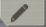
\includegraphics[width=0.05\textwidth]{butt_pencil.png} on the top right corner of a simulation tab. From the menu you can get a copy, edit the name the simulation or delete it. (Fig. \ref{fig:sim_copy}).
\item Change the name of the new simulation (e.g., \textit{AnatomyOfARegionSimulation\_b} ) and set the coupling strength to the value in step 1. Launch the simulation.
\end{enumerate}
\end{simulation}


Looking at the time series of \textit{AnatomyOfARegionSimulation\_b}, we can see that the system exhibits self-sustained
oscillations. 

\begin{figure}[h]
  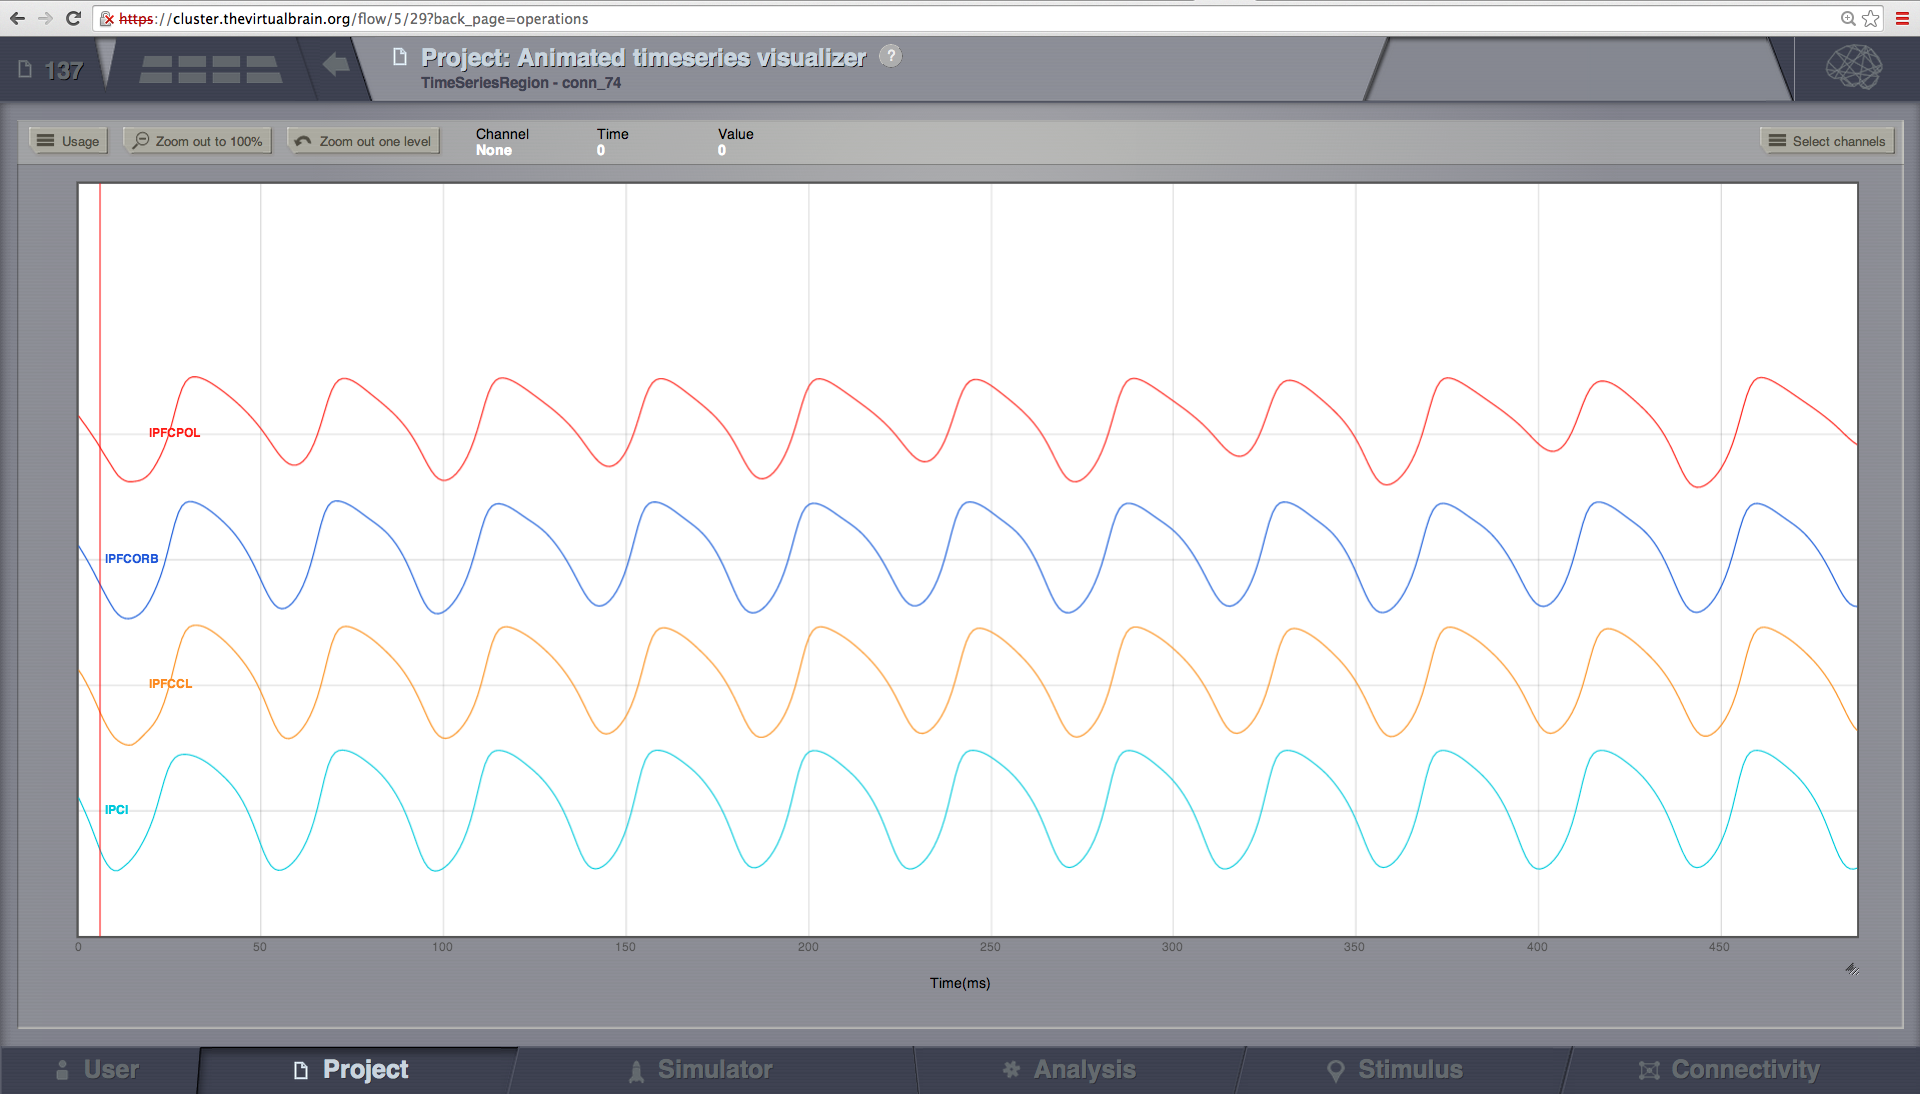
\includegraphics[width=\linewidth]{Handout_UI_BuildingYourOwnBrainNetworkModel_AnimatedTimeSeriesOscillatory}%
  \caption{Time-series from \textit{AnatomyOfARegionSimulation\_b}}%
  \label{fig:time_series_oscillatory}%
\end{figure}


A frequent question is at which value of coupling strength this
"bifurcation" occurs. Well, we can easily set up a parameter search by defining a
range of values that will be explored. We'll see how to do this in the next section.

 \newpage
\subsection{Parameter Space Exploration (PSE)}\label{sec:pse}

\newthought{TVB will launch a simulation} for
every value. \sidenote{For the time being, parameter space explorations are restricted to
two dimensions.} The example is set up in \textit{AnatomyOfARegionSimulation\_pse\_a}. 

\begin{simulation}
\begin{enumerate}
 \item In \underline{Long range coupling function}, under \textbf{a}, click on 
\includegraphics[width=0.1\textwidth]{butt_expand_range.png}. 
 Set the range between $\mathbf{0.012 \text{ and } 0.042}$ and the step to $\mathbf{0.002}$.
 \item Do the same under \underline{conduction speed}, setting the range between $\mathbf{1-10}$ \unitfrac{mm}{ms} and the step to \textbf{\unitfrac[1]{mm}{ms}}.
 
 \item Set the \underline{simulation length} to \textbf{\unit[2000]{ms}} and launch the simulations.
\end{enumerate}
\end{simulation}

\begin{marginfigure}
  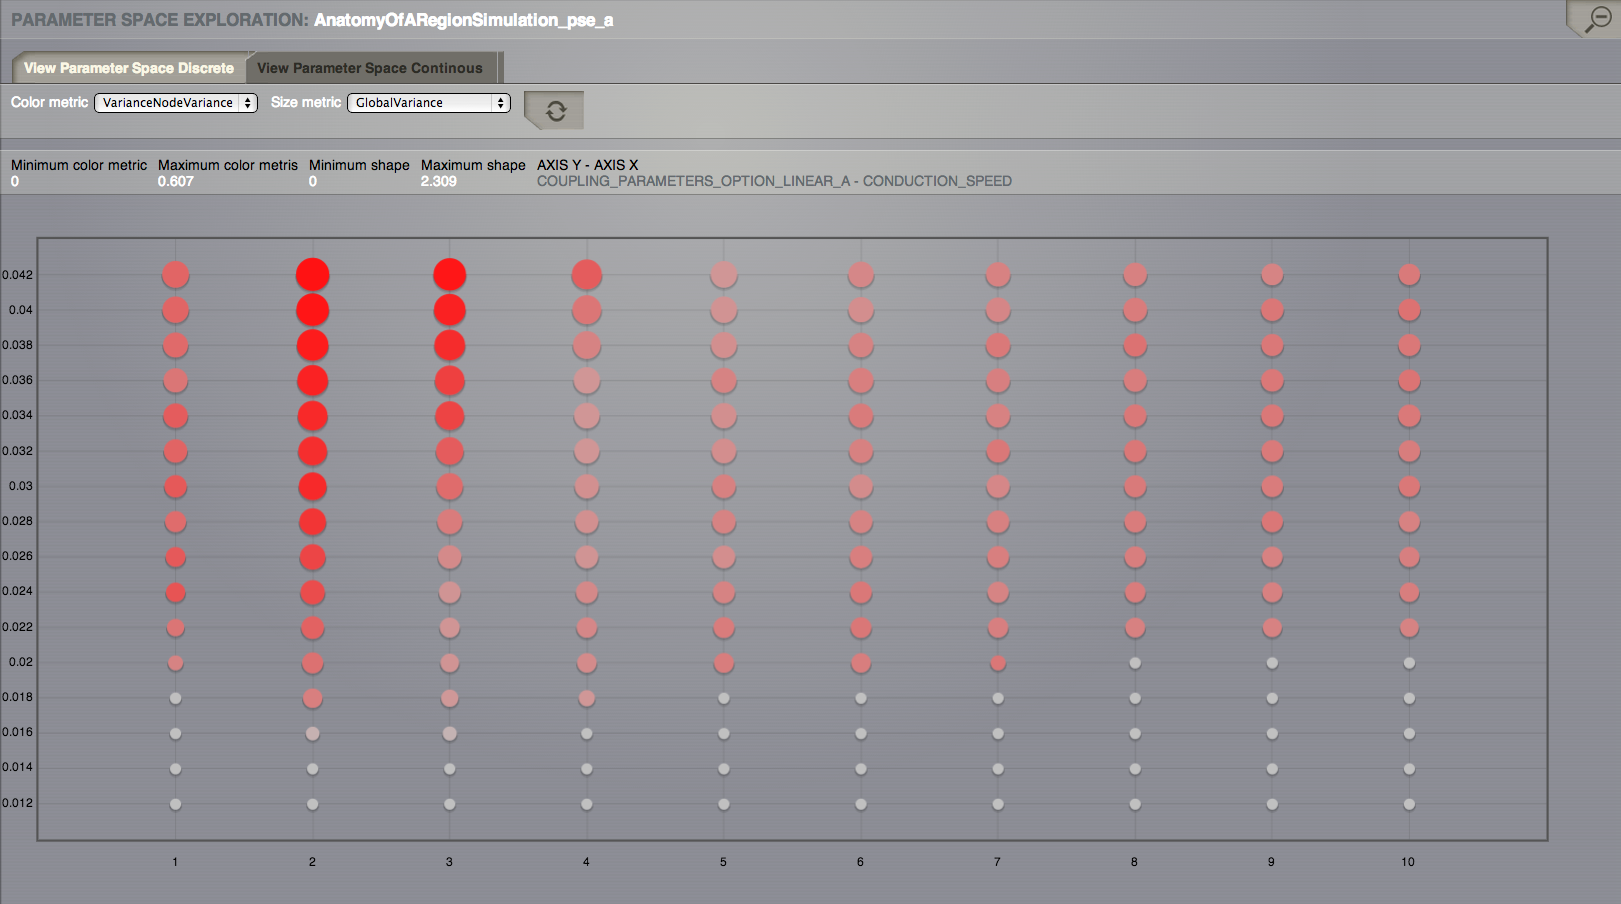
\includegraphics[width=\linewidth]{Handout_UI_BuildingYourOwnBrainNetworkModel_PSEDiscrete}%
  \caption{Discrete parameter space map from \textit{AnatomyOfARegionSimulation\_pse\_a}}%
  \label{fig:pse_discrete}%
\end{marginfigure}

\begin{marginfigure}
  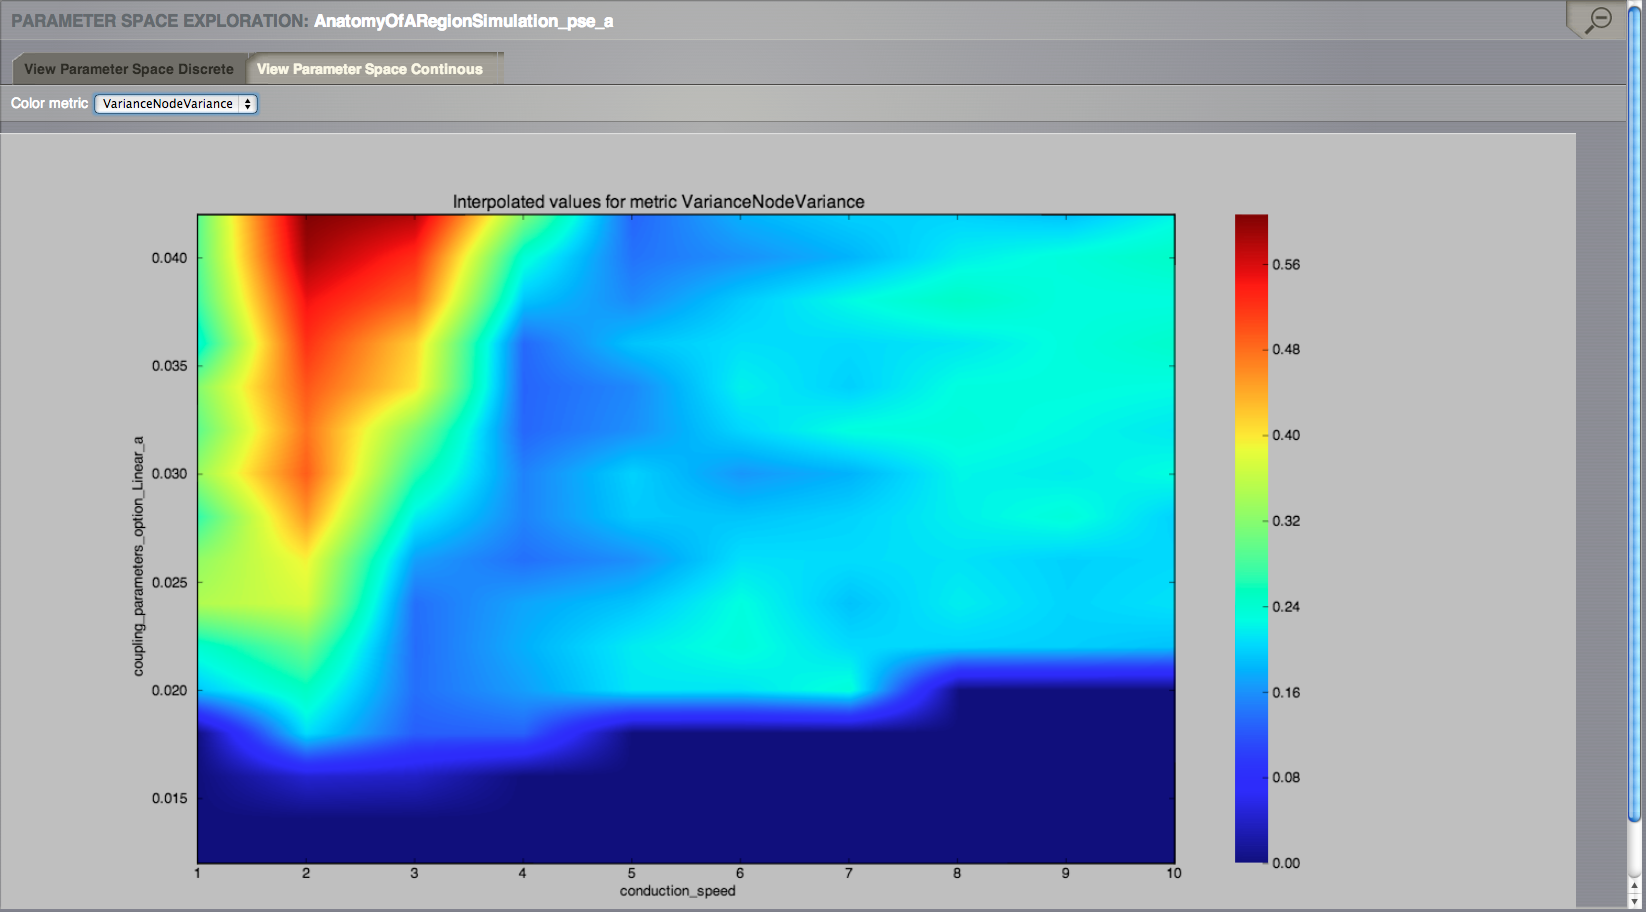
\includegraphics[width=\linewidth]{Handout_UI_BuildingYourOwnBrainNetworkModel_PSEContinuous}%
  \caption{Continuous parameter space map from \textit{AnatomyOfARegionSimulation\_pse\_a}}%
  \label{fig:pse_continuous}%
\end{marginfigure}

All the 150 simulations are presented as a discrete 2D map in \underline{Parameter Space Discrete} \sidenote{Each point represents a simulation. The size and the colour of the marker correspond to one of a few variance metrics implemented to have an idea of the network node and temporal variability.} (Fig. \ref{fig:pse_discrete}) or a continous pseudocolor map in \underline{Parameter Space Continous}\sidenote{The colour scale  corresponds to one of the variance metrics} (Fig. \ref{fig:pse_continuous}). 




\begin{blah}
 These results are those presented in \citep{Ghosh_2008} and \citep{Knock_2009}. 
\end{blah}

\subsection{Simulation continuation or Branching}\label{sec:results}

\newthought{Other parameters could be} adjusted as well. We mentioned before
that the big transient at the beginning of the time-series is due to the initial conditions. To
overcome this issue we have a couple of alternatives. First, we could narrow the range of the state variables around the values of a fixed point. How can we know this value?. \sidenote{go back to the \textsc{simulator} page and load either \textit{AnatomyOfARegionSimulation\_a} or \textit{AnatomyOfARegionSimulation\_b}}.

\begin{simulation}
\begin{enumerate}
\item  Clik on \underline{Set up region model}, you'll be redirected to a new working area. 
\end{enumerate}
\end{simulation}


In this area there's a an interactive tool, the \underline{Phase Plane}, which allows you to understand the local dynamics, that is the dynamics of a single isolated node, by observing how the model parameters change its phase plane. (See Fig. \ref{fig:ppi}).

\begin{marginfigure}%
  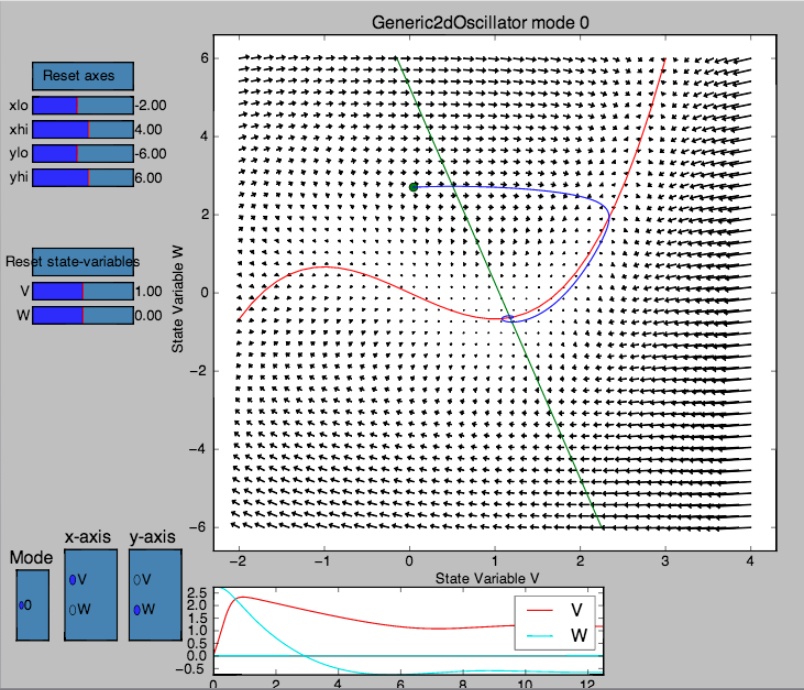
\includegraphics[width=\linewidth]{Handout_UI_BuildingYourOwnBrainNetworkModel_PhasePlane}%
  \caption{Phase Plane Interactive}%
  \label{fig:ppi}%
\end{marginfigure}%

\begin{simulation}
\begin{enumerate}[resume]
  \setcounter{enumi}{1}
\item  Click on any point of the phase plane. A trajectory will be drawn.
We see that the fixed point is approx (V, W) = (1.5, -0.6)
\end{enumerate}
\end{simulation}


However, there certainly is a more elegant way. 

\begin{simulation}
\begin{enumerate}[resume]
 \setcounter{enumi}{2}
\item Set your model with fixed point dynamics and a weak coupling strength (e.g., \textit{AnatomyOfARegionSimulation\_a})
\item Run a simulation for \textbf{\unit[1000]{ms}}.
\end{enumerate}
\end{simulation}

TVB has a branching mechanism that allows you to use the data of a simulation, as the initial history for a new simulation. The only thing you
need to know is that the spatio-temporal structure of the network should
remain unchanged (e.g., the number of nodes, conduction speed, the recorded state-variables, integration time-step size and selected monitors should be the same.)

\begin{simulation}
\begin{itemize}[resume]
 \setcounter{enumi}{4}
 \item In \textit{AnatomyOfARegionSimulation\_a}, set $\mathbf{a=0.042}$ in the \underline{long range coupling function}. Then, click on 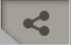
\includegraphics[width=0.05\textwidth]{butt_branching.png}. 
\end{itemize}
\end{simulation}

\textit{AnatomyOfARegionSimulation\_a\_branch1} is an example of this functionality, using the results from \textit{AnatomyOfARegionSimulation\_a} as initial conditions. 

\subsection{Stochastic Simulations}\label{sec:noisy_simulations}


As a last point, we will show the basics of running a simulation driven by
noise (i.e., using a stochastic integration scheme \sidenote{We can choose between \underline{Additive} and \underline{Multiplicative Noise} functions when defining
the way noise enters our simulation. In the case of \underline{Multiplicative Noise} the
function depends on the state of the system.}). Here we'll also use a region
level simulation, but the considerations for surface simulations are the same.
In a stochastic integration scheme \underline{Noise} enters through the integration
scheme. 

\begin{blah}
\begin{itemize}
Here we'll define a simple constant level of noise that enters all
nodes and all state variables, however, the noise is configurable on a per
node and per state variable level, and as such the noise can be reconfigured
to, for example, only enter appropriate state variables of certain thalamic
nodes, thus emulating a very crude model of external inputs to the brain. 
\end{itemize}
\end{blah}

\begin{simulation}
\begin{enumerate}
\item After configuring a model similar to the one presented in  \textit{AnatomyOfARegionSimulation\_b}, we select \textbf{HeunStochastic} as an integration scheme.  
\end{enumerate}
\end{simulation}

The \underline{Noise} functions are fed by a
random process generated by a pseudo-random number generator (PRNG). The random
processes used have Gaussian amplitude and can potentially be given a temporal
correlation. The random process is defined using two
parameters plus the seed of the PRNG. The two parameters are: $\mathbf{D}$ \sidenote{As a general rule of thumb, the noise
amplitude, when being applied to all nodes and all state-variables, should be
much less than 1\% of the expected state-variable range if you don't want the
noise to dominate the intrinsic dynamics of the system.
If you are not sure about the level of noise, using the Phase Plane
Interactive tool for plotting noisy trajectories is a good place to start. See Fig. \ref{fig:ppi_noise}}, defining the
standard deviation of the noise amplitude; and $\boldsymbol{\tau}$ which defines the
correlation time of the noise source, with $\boldsymbol{\tau = 0}$ corresponding to white
noise and any value greater than zero producing coloured noise. 

\begin{marginfigure}%
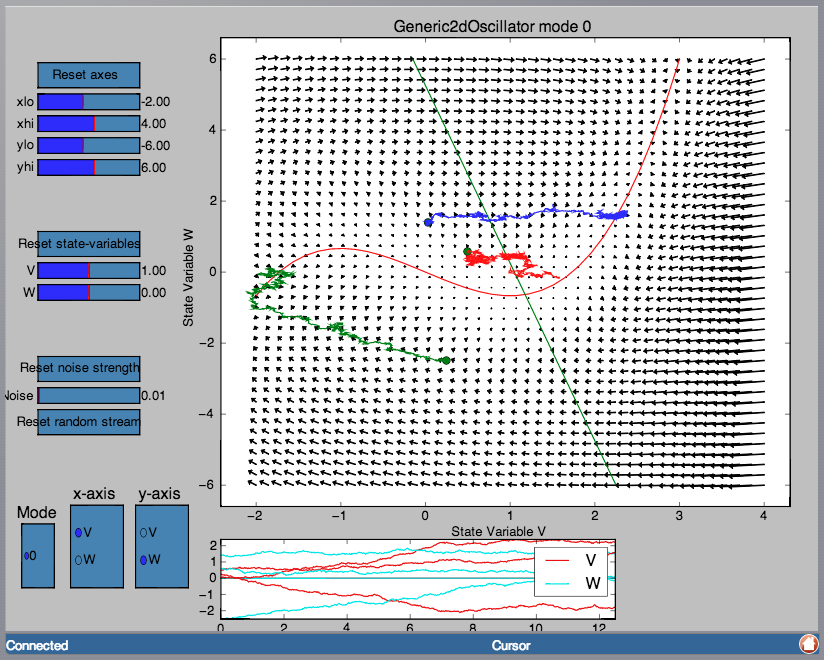
\includegraphics[width=\linewidth]{Handout_UI_BuildingYourOwnBrainNetworkModel_PPI}%
  \caption{Stochastic trajectories}%
  \label{fig:ppi_noise}%
\end{marginfigure}

\begin{simulation}
\begin{enumerate}[resume]
\setcounter{enumi}{1}
\item After configuring a model similar to the one presented in  \textit{AnatomyOfARegionSimulation\_b}, we select \textbf{HeunStochastic} as our integration scheme.  
\item Set the values for {$\boldsymbol{\tau=0}$}  and \textbf{seed=42}. 
\item Set the noise dispersion, $\mathbf{D=0.005}$
\end{enumerate}
\end{simulation}
%\newpage
\textit{AnatomyOfARegionSimulation\_b} and \textit{AnatomyOfARegionSimulation\_c} have the same parameters but the latter has an extra background noisy input. 

\begin{formal}
\begin{enumerate}
Observe the differences using the \underline{Spectrogram of the Wavelet Transform}. Figs. \ref{fig:wavelet_deteministic} and \ref{fig:wavelet_stochastic}
\end{enumerate}
\end{formal}

\begin{marginfigure}%
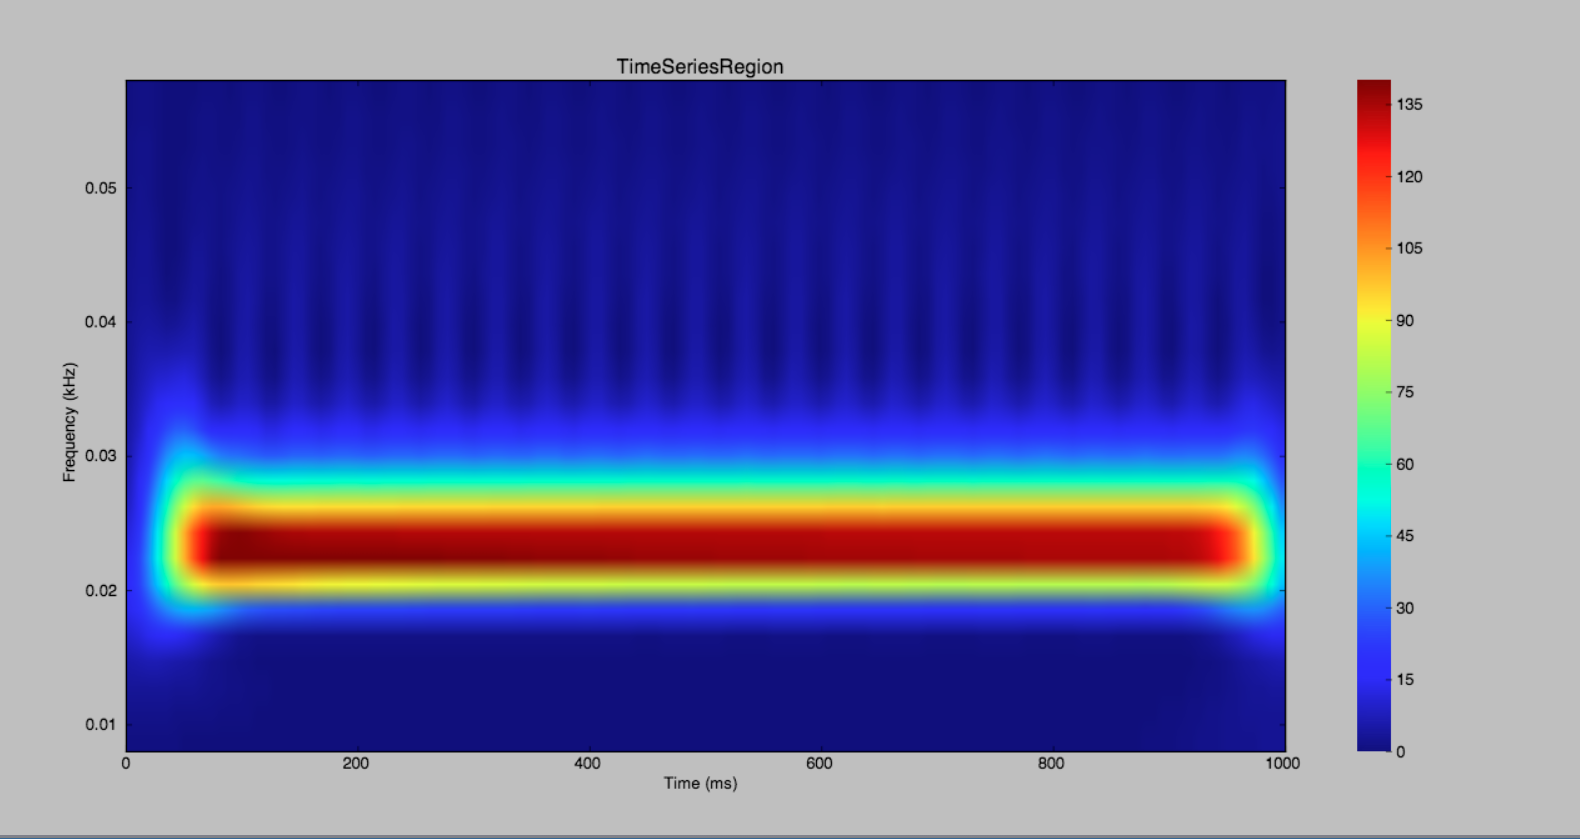
\includegraphics[width=\linewidth]{Handout_UI_BuildingYourOwnBrainNetworkModel_WaveletDeterministic}%
  \caption{Spectrogram of the wavelet transform from \textit{AnatomyOfARegionSimulation\_b}}%
  \label{fig:wavelet_deteministic}%
\end{marginfigure}
%
\begin{marginfigure}%
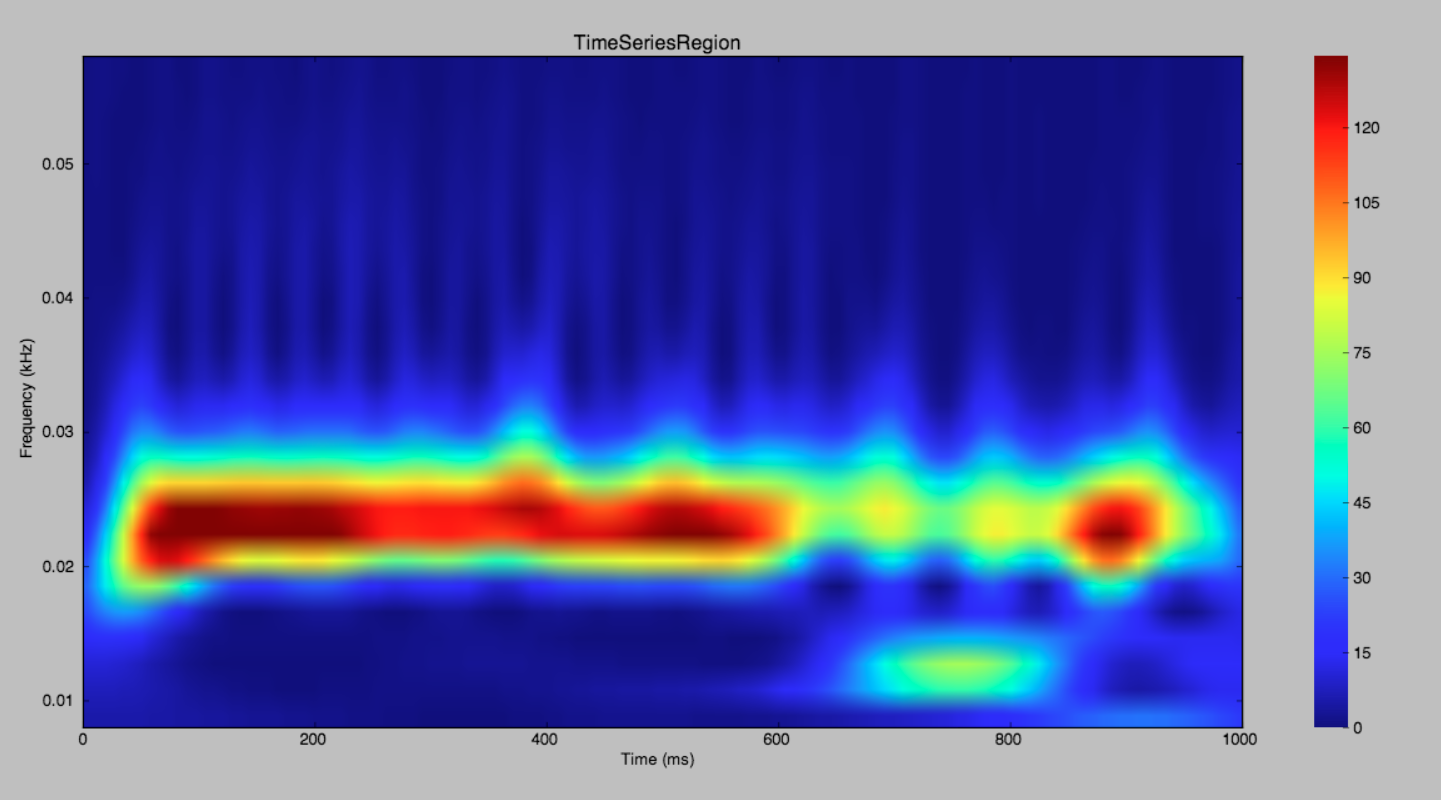
\includegraphics[width=\linewidth]{Handout_UI_BuildingYourOwnBrainNetworkModel_WaveletStochastic}%
  \caption{Spectrogram of the wavelet transform from \textit{AnatomyOfARegionSimulation\_c}}%
  \label{fig:wavelet_stochastic}%
\end{marginfigure}


\subsection{Extra}\label{sec:results}

If you are already anxious and wondering about fMRI and some other biophysical output modalities, in \textit{AnatomyOfARegionSimulation\_d\_branch1} we've generated \unit[4]{min} worth of data using a convolution based model of the BOLD signal (see Fig. \ref{fig:BOLD}). Load this simulation if you want to see the parameter values.

\begin{marginfigure}%
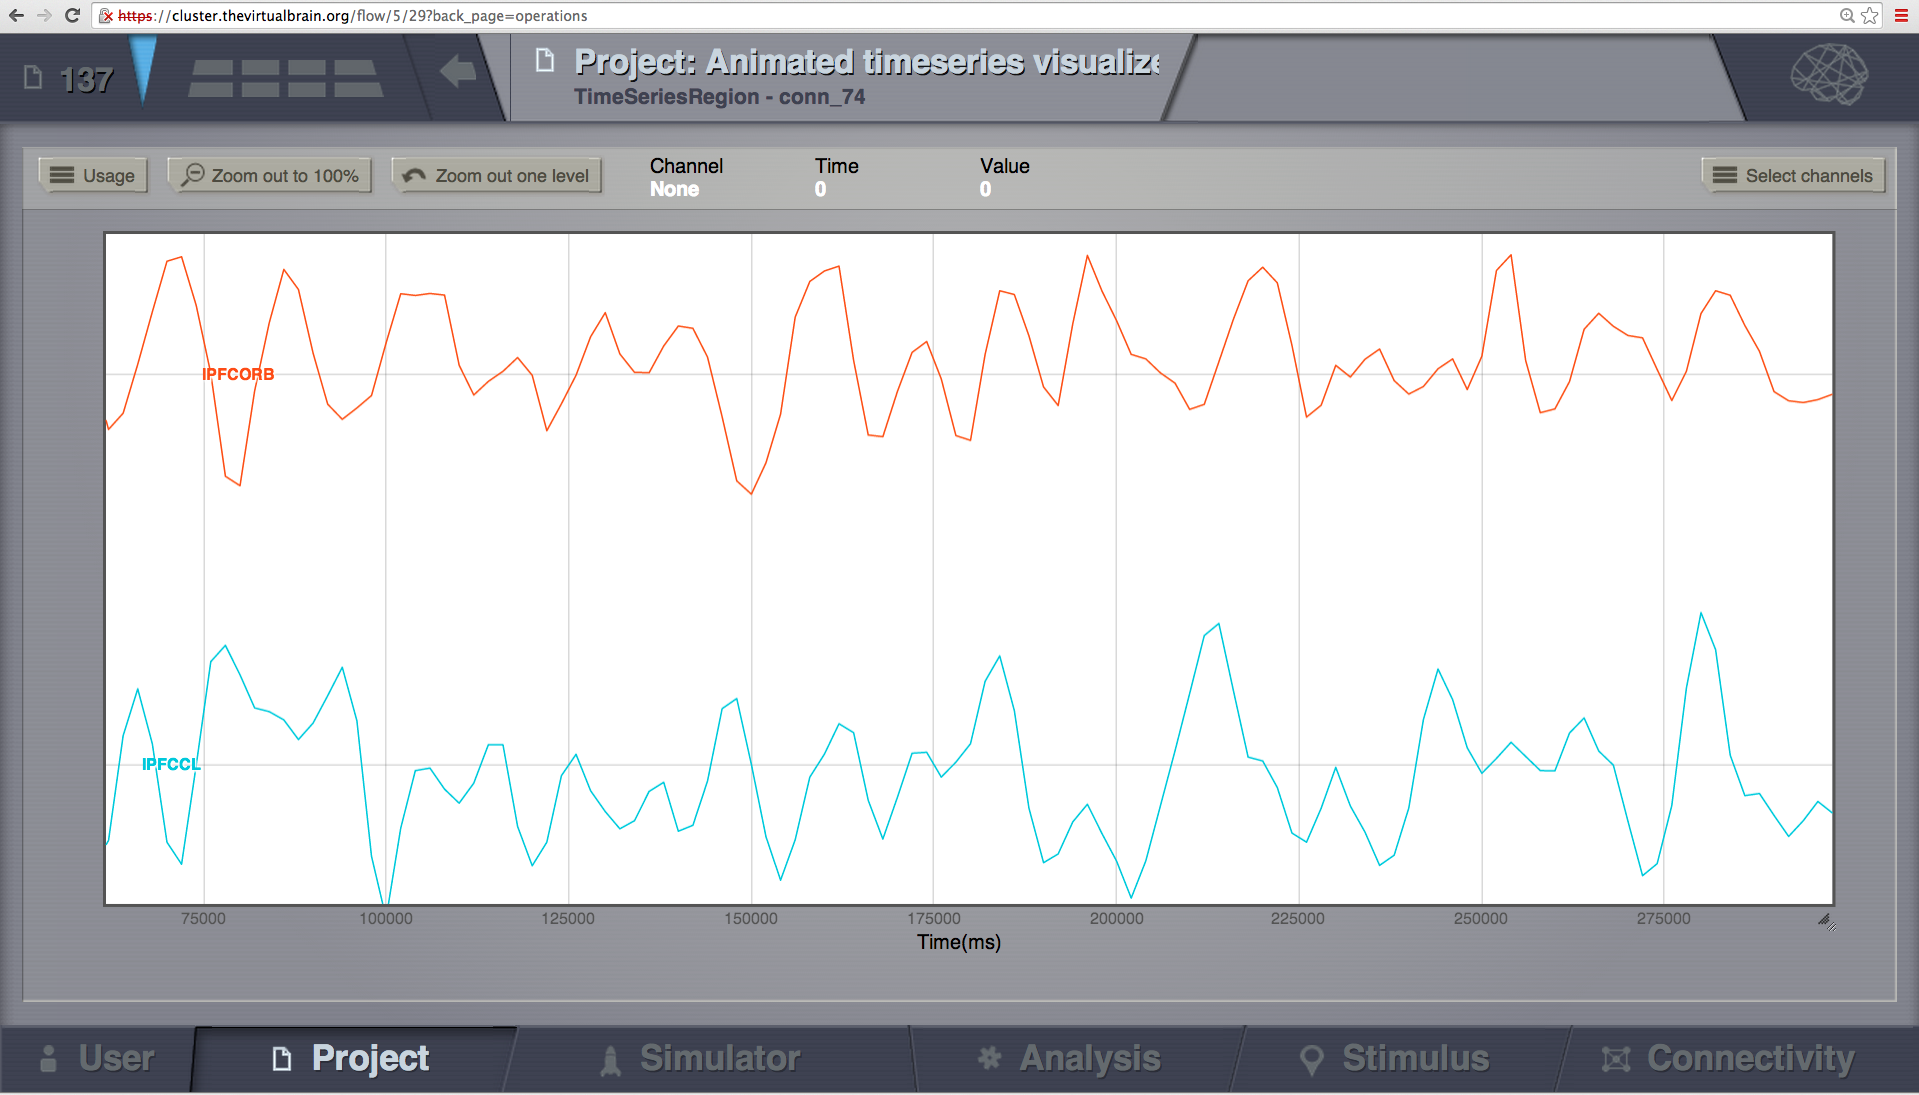
\includegraphics[width=\linewidth]{Handout_UI_BuildingYourOwnBrainNetworkModel_BOLD}%
  \caption{BOLD signals from \textit{AnatomyOfARegionSimulation\_d\_branch1}}%
  \label{fig:BOLD}%
\end{marginfigure}

\newpage
\subsection{Modelling the Neural Activity on the Folded Cortex}\label{sec:surface_simulations}

This extends the basic region simulation to include the folded cortical surface to the anatomical structure on which the simulation is based. If you haven't read or followed was written above you probably should do that now as here we only really discuss in detail the extra components that are specific to a simulation on the cortical surface.

\begin{blah}
In addition to the components discussed for a
region simulation here we introduce two major components, that is:
\begin{itemize}
\item \underline{Cortical Surface}, which is a mesh surface defining
a 2d representation of the convoluted cortical surface embedded in 3d space.
\item \underline{Local Connectivity}, that represents the probability of the interactions between neighbouring nodes on a local patch. 
\item \underline{Region Mapping},  a breakup that defines to which anatomical region in the \underline{Connectivity} each vertex of the mesh belongs to. 
\end{itemize}
\end{blah}

\begin{simulation}
\begin{enumerate}
\item The \underline{connectivity}, \underline{speed}, \underline{coupling strength} and \underline{local model} and its parameters are the same described in  \textit{AnatomyOfARegionSimulation\_b} and Table \ref{tab:modeltab}.
\item Select the \textbf{TVB's default Cortical Surface}, which has 16384 nodes. 
\item We rely on \textbf{TVB's default Local Connectivity}.
\item Rescale the \underline{Local Connectivity} with \underline{Local coupling strength} equal to $\mathbf{0.1}$.
\item For the integration we'll use \textbf{HeunDeterministic}.  Here, integration time step size is the default: $\mathbf{dt=}$\textbf{\unit[0.1220703125]{ms}}.
\end{enumerate}
\end{simulation}

The first significant thing to note about surface simulations is that certain \underline{Monitors} make a lot more sense in this context than they do at the region level, and so we'll introduce a couple new \underline{Monitors} here.

\begin{marginfigure}
 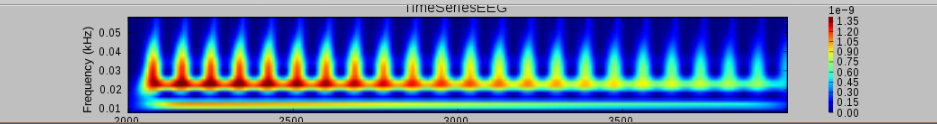
\includegraphics[width=\linewidth]{Handout_UI_BuildingYourOwnBrainNetworkModel_DefaultLocalConnectivityWaveletSpectrogram.png}%
  \caption{Spectrogram of the spatially averaged time-series from \textit{AnatomyOfASurfaceSimulation\_branch1}.}%
  \label{fig:default_lc_spectrogram}%
\end{marginfigure}



\begin{marginfigure}
  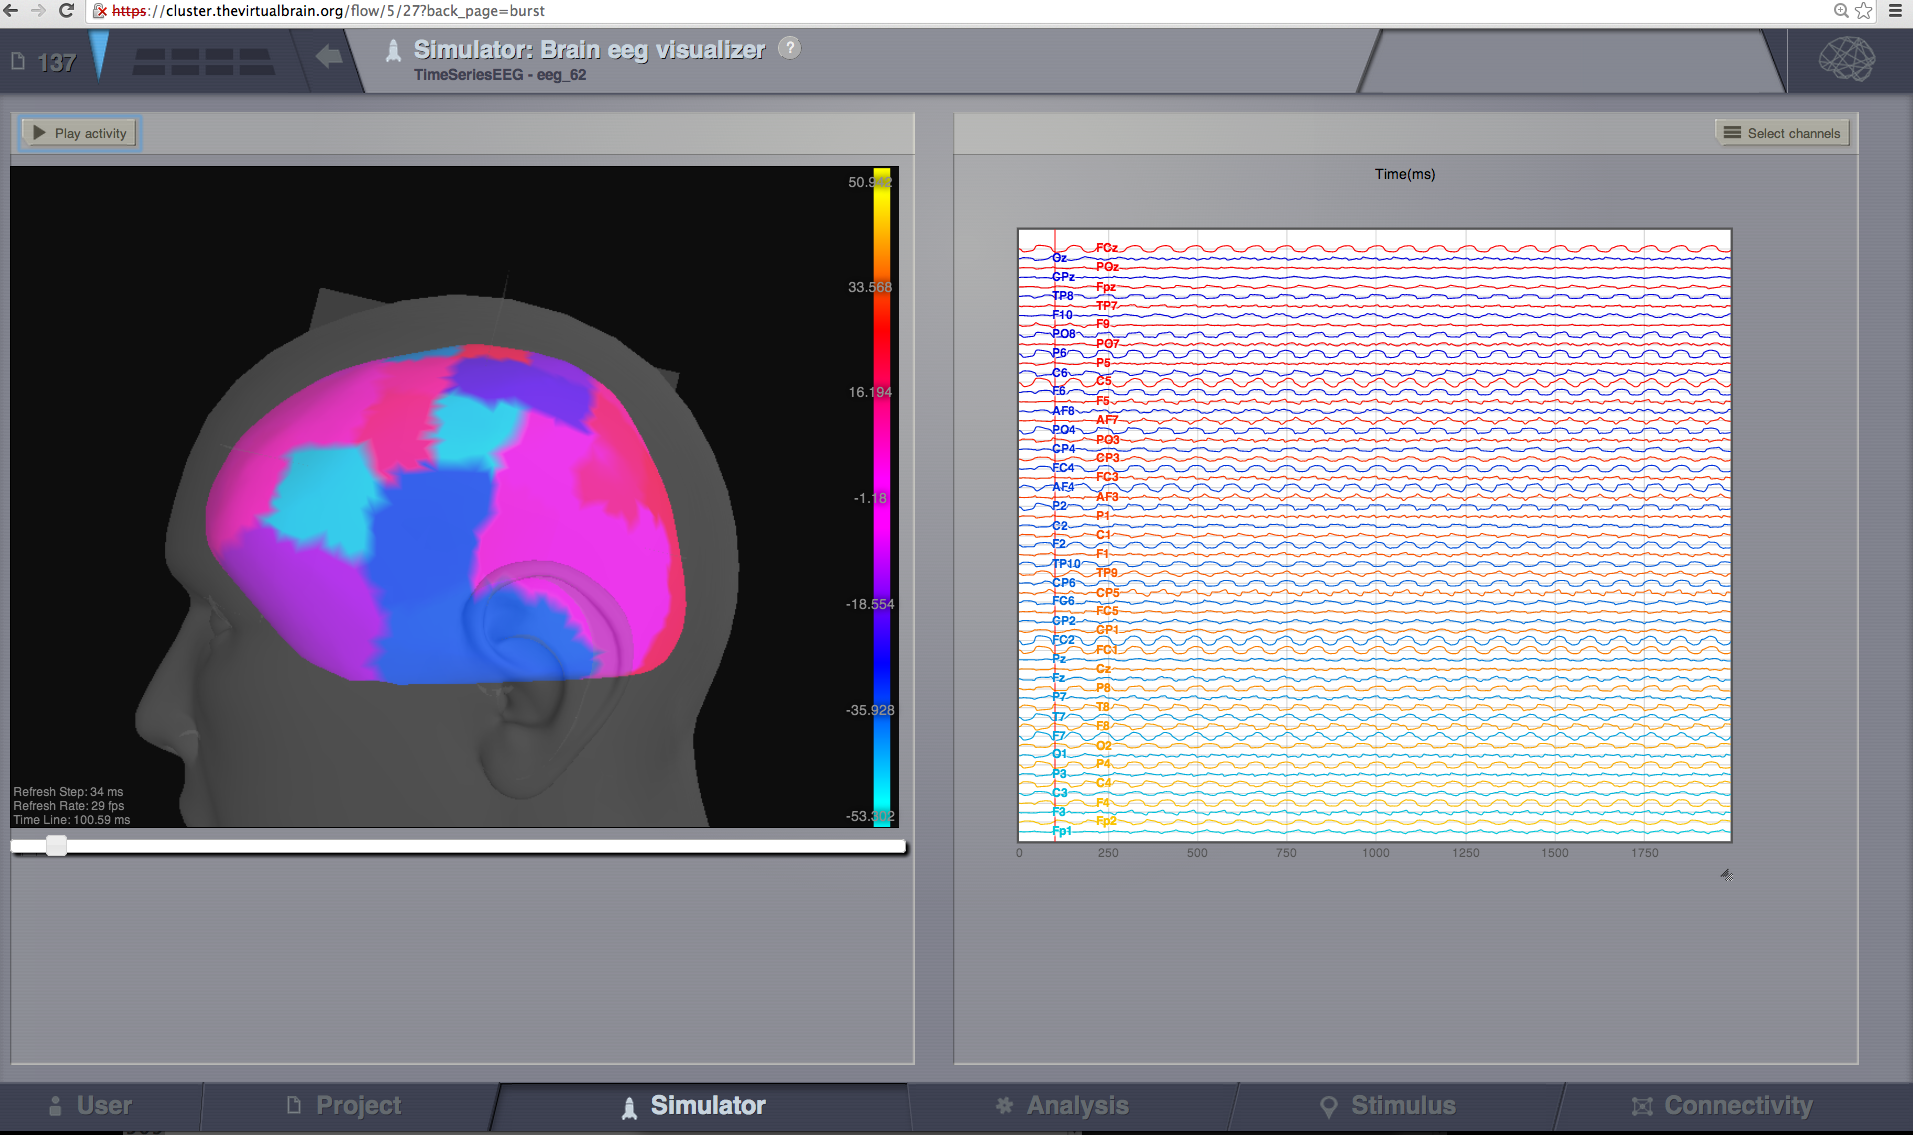
\includegraphics[width=\linewidth]{Handout_UI_BuildingYourOwnBrainNetworkModel_MexicanLocalConnectivityPotatoHead.png}%
  \caption{EEG signals from \textit{SurfaceSimulation\_MexicanHatLocalConnectivity}}%
  \label{fig:potato_head}%
\end{marginfigure}

\begin{simulation}
\begin{enumerate}[resume]
\setcounter{enumi}{5}
\item The first of these new \underline{Monitors} is called
\textbf{{SpatialAverage}}. To select several monitors press the key Command or Control while you select them.
\item The second of these new monitors, which is an instantiation of a
biophysical measurement process, is called \textbf{EEG}. 
\item The \underline{Monitors period} is left with the default value \textbf{\unit[0.9765625]{ms}} which is equivalent to a sampling frequency of \unit[512]{Hz}.
\item Lastly, the \underline{simulation length} is \textbf{\unit[2000]{ms}}.
\item Run the simulation.
\item Once the simulation is finished, without changing any parameters, click on 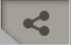
\includegraphics[width=0.08\textwidth]{butt_branching}.

\end{enumerate}
\end{simulation}


These simulations are \textit{AnatomyOfASurfaceSimulation} and \textit{AnatomyOfASurfaceSimulation\_branch1}. In Fig. \ref{fig:default_lc_spectrogram} you can see the spectrogram of the wavelet transform of the spatially averaged time-series from 
the simulation \textit{AnatomyOfASurfaceSimulation\_branch1}. 



The first of these new \underline{Monitors},  will average over the
space (nodes) of the simulation. \sidenote{In the case of region level simulations we
already have a situation of a relatively small number of nodes, with each one
representing a fairly large chunk of brain. In surface simulations on the
other hand we can easily have tens of thousands of nodes, and reducing this by
averaging over sensible collections of these nodes can be valuable.} The basic
mechanism is general, in the sense that the nodes can be broken up into any
non-overlapping, complete, set of sets. In other words, each node can only
be counted in one collection and all nodes must be in one collection. \sidenote{In fact
this is the default behaviour of the \underline{Spatial Average} monitor when
applied to a surface simulation, that is it averages over nodes and returns
region based time-series. } 



%An alternative is to spatially average the signals
%according to the hemisphers the nodes belong two.  When applied to region
%simulation distinct spatial masks, or index vectors, can be used such as
%\underline{hemispheres} which, as you may guess, will average the left nodes
%and right nodes separetly resulting in two time-series; and,
%\underline{cortical}, which will average all the cortical nodes and those
%repsresenting subcortical structuresin two different time series.


The second of these new Monitors, \underline{EEG}, hopefully also
unsurprisingly, returns the EEG signals resulting from the simulated neural
dynamics using in the process a lead-field or \underline{Projection Matrix}. \sidenote{The EEG monitor will return a relatively standard 62 channel set based on the
10-20 system.} 



\begin{blah}
EEG signals measured on the scalp depend strongly on the location
and orientation of the underlying neural sources, which is why this monitor is
more realistic and useful in the case of surface based simulations -- where
the simulation is run on the explicit geometry of the cortex, which can
potentially have been obtained from a specific individual's brain. 
In addition a simulation being built on the specific anatomical structure of an individual
subject, the specific electrodes used in experimental work can also be
incorporated, providing a link between simulation and
experiment. See Fig. \ref{fig:potato_head}
\end{blah}

\subsection{Define Your Own Local Connectivity}\label{sec:local_connectivity}

The regularized mesh can support, in principle, arbitrary forms for the
\underline{local connectivity kernel}. Coupled across the realistic surface geometry this
allows for a detailed investigation of the local connectivity's effects on
larger scale dynamics modelled by neural fields.



\begin{formal}
\begin{enumerate}
\item Go to \textsc{Connectivity} $\rightarrow$ \textsc{Local Connectivity}. 
In this area we'll build two different kernels: a Gaussian and a Mexican Hat kernel. 
We'll start with the Gaussian kernel. 
\item Select the \underline{equation defining the spatial profile} of your \underline{local connectivity}. Here, we'll leave the defaults.
\item Select a \underline{cutoff distance}, that is, the distance up to which a given node is connected to its neighbourhood \citep{Spiegler_2013, Sanz-Leon_2014}. Ideally, you want the function to have essentially dropped to zero by the \textbf{cutoff distance}. Here this value is set to \textbf{\unit[40]{mm}}. See Fig. \ref{fig:lc_gaussian}.
\item Name your \underline{Local connectivity} and save it by clicking on \underline{Create new Local Connectivity} on the bottom left corner. 
\end{enumerate}
\end{formal}
This data structure is saved under the name \textit{LocalConnectivity\_Gaussian\_zc\_40}.

\begin{figure}[h]
  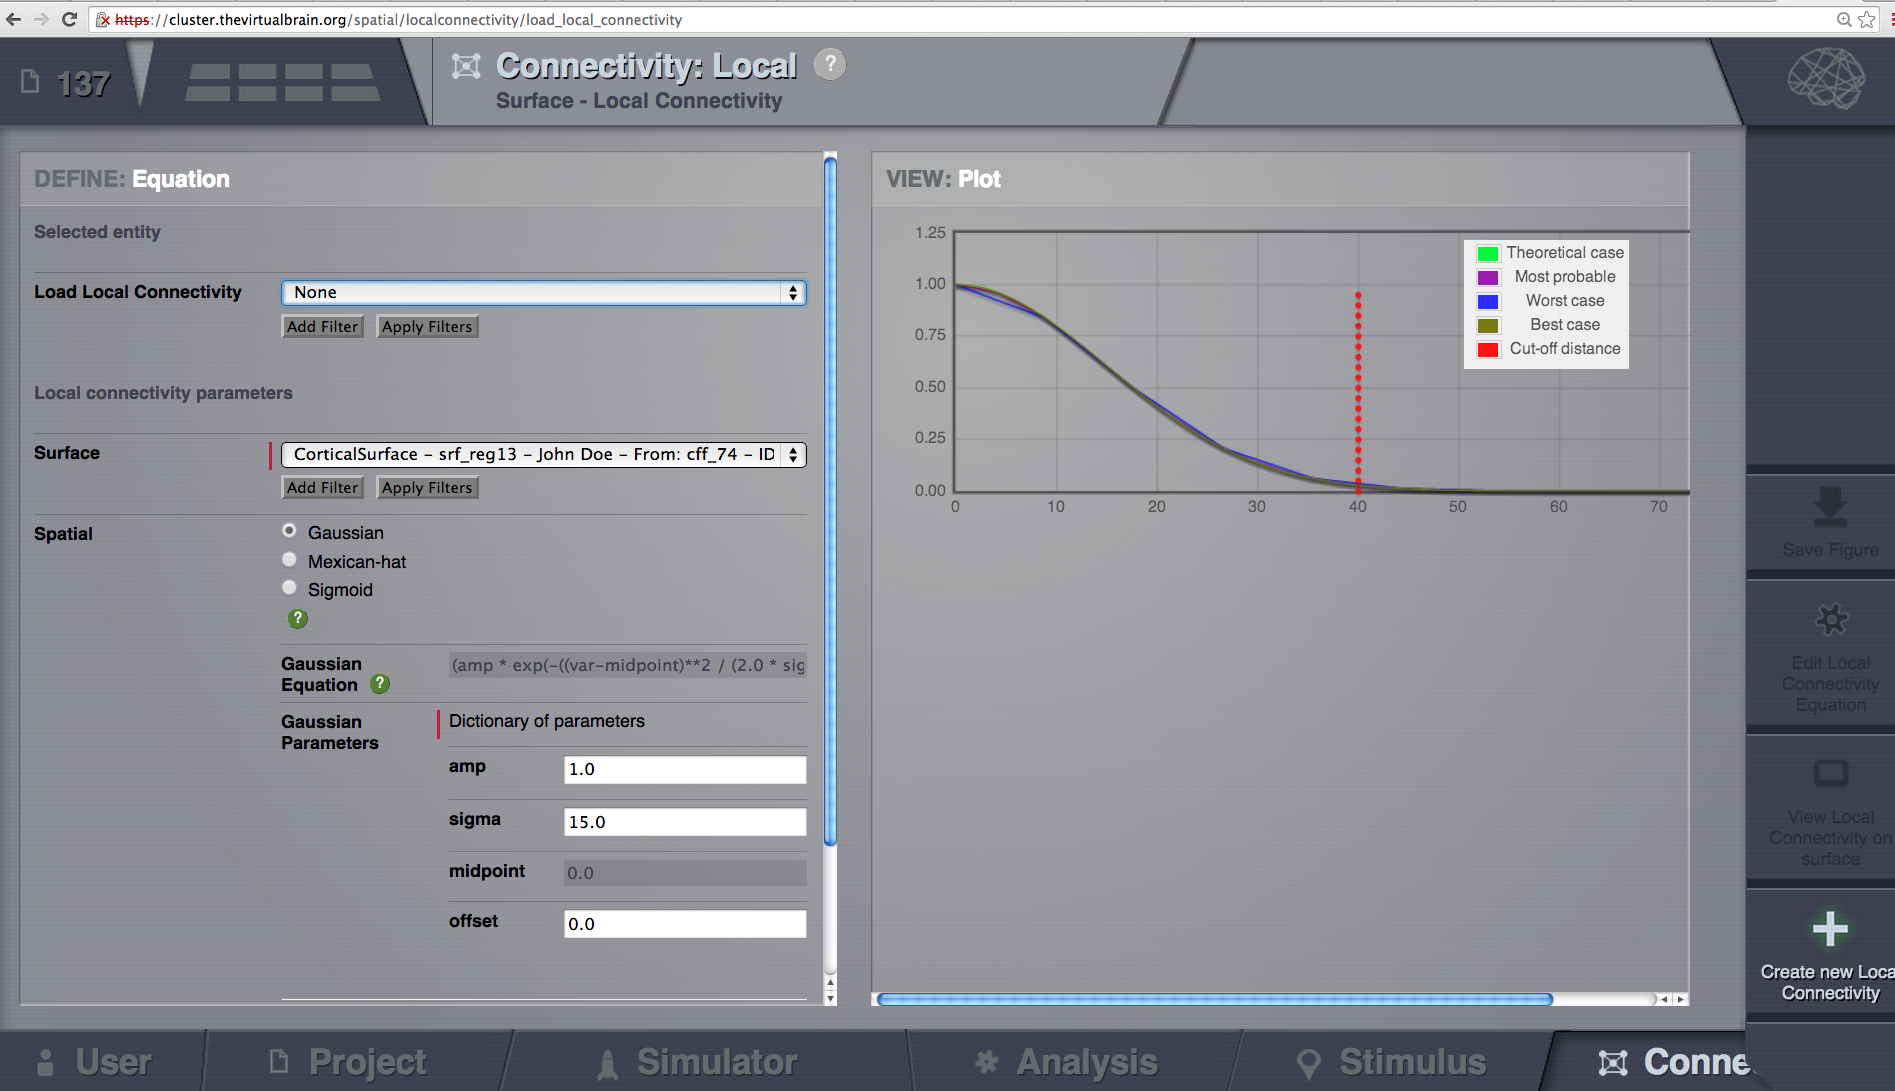
\includegraphics[width=\linewidth]{Handout_UI_BuildingYourOwnBrainNetworkModel_YourOwnLocalConnectivity}%
  \caption{Gaussian local connectivity. We have on the right a representation of the kernel for a quick idea of how
the \underline{Local Connectivity} we've just specified will be represented on the
surface. This plots the local connectivity function with different sampling
based on the distribution of edge lengths in your mesh surface. If all the
lines don't, at least mostly, overlap then you've probably specified a
function with structure that is too fine for the resolution of your mesh
surface. }%
  \label{fig:lc_gaussian}%
\end{figure}




\begin{formal}
\begin{enumerate}[resume]
\setcounter{enumi}{4}
\item Select the \underline{Mexican Hat equation}. Here, we changed the default parameters. See the values in Table \ref{tab:mexicanstab}.
\item Save your new local connectivity.
\end{enumerate}
\end{formal}

This data structure is saved under the name \\
\textit{LocalConnectivity\_MexicanHat\_zc\_40}.


\begin{margintable}
  \centering
  \fontfamily{ppl}\selectfont
  \begin{tabular}{ll}
    \toprule
    Parameter & Value \\
    \midrule
             midpoint\_1          &   \unit[0]{mm}\\
             midpoint\_2          &   \unit[0]{mm}   \\
             amp\_1                 &   \unit[2]{au}        \\
             amp\_2                 &   \unit[1]{au}        \\
             sigma\_1          &   \unit[5]{mm}   \\
             sigma\_2          &   \unit[15]{mm}   \\
             cutoff distance & \unit[40]{mm}\\
    \bottomrule
  \end{tabular}
  \caption{\textit{LocalConnectivity\_MexicanHat\_zc\_40} parameters. }
  \label{tab:mexicanstab}
\end{margintable}


\begin{simulation}
\begin{enumerate}[resume]
\setcounter{enumi}{4}
\item Finally, we run two  more simulations, using the same parameters described in \textit{AnatomyOfASurfaceSimulation}, but using  \textbf{\textit{LocalConnectivity\_MexicanHat\_zc\_40}} in one case and  \textbf{\textit{LocalConnectivity\_Guassian\_zc\_40}} in the other case. The \textbf{local connectivity strength} is set to \textbf{-0.001}. 

\end{enumerate}
\end{simulation}

These results are those of \textit{SurfaceSimulation\_MexicanHatLocalConnectivity} and \textit{SurfaceSimulation\_GaussianLocalConnectivity} respectively.
 

\section{More Documentation}\label{sec:more-doc}
And that's it for this session, while the simulations are not particularly scientifically
interesting, hopefully it gave you a sense of the anatomy of a
simulation within TVB and many of the configurable parameters and output
modalities. Online help is available clicking on the 
\includegraphics[width=0.05\textwidth]{butt_green_help} icons next to each entry.
For more documentation on The Virtual Brain, please see the following articles \citep{Ghosh_2008, Sanz-Leon_2013, Spiegler_2013, Woodman_2014, Jirsa_2010b}


\section{Support}\label{sec:support}

The official TVB webiste is \url{www.thevirtualbrain.org}.  
All the documentation and tutorials are hosted on \url{the-virtual-brain.github.io}.
You'll find our public \smallcaps{git} repository at \url{https://github.com/the-virtual-brain}. 
For questions and bug reports we have a users group \url{https://groups.google.com/forum/#!forum/tvb-users}

\bibliography{tvb_references}
\bibliographystyle{plainnat}

\end{document}